\chapter{Lattice study of a gauge-fermion-scalar theory}

The Standard Model electroweak theory is very successful in describing experimental results. However, some theoretical concerns suggest that a more consistent theory should be found. Specifically, the search for an alternative mechanism for the generation of masses is an active research field.
Composite Higgs models belong to this branch of Beyond the Standard Model (BSM) research.

In this chapter we discuss the lattice study of an SU(2) gauge theory coupled to fermions and scalars. This theory is intended as a minimal scenario for composite Higgs models, in which the problem of the generation of fermion masses is addressed via the fundamental partial compositeness mechanism \cite{Sannino:2016sfx}. 

The chapter is organised as follows. We start by exposing some of the reasons why the Standard Model Higgs mechanism turns out to be theoretically unappealing. Then we introduce composite Higgs models, and we explain what makes the generation of fermion masses a bit problematic in this setup. We then describe the mechanism of fundamental partial compositeness.
After setting these theoretical motivations, we move to the description of the specific theory under analysis, starting with some continuum aspects and then moving to the lattice setup. Finally,  we present the results obtained on the spectrum and phase space of the lattice theory. Some of these results have been published in \cite{Hansen:2017mrt}, while others are reported here for the first time.


%%%%%%%%%%%%%%%%%%%%%%%%%%%%%%%%%%%%%%%%%%%%%%%%%%

\section{Composite Higgs models and fundamental partial compositeness}


\subsection{The naturalness and triviality problems}

The Standard Model Higgs boson is an elementary scalar field. There exist some theoretical problems related to elementary scalars, known as naturalness and triviality problem. 

The naturalness problem is due to the fact that the Higgs mass is extremely sensitive to corrections arising from new physics, which may appear at a very high energy scale. We know the Standard Model to be an effective field theory, valid up to some ultraviolet cutoff $\Lambda_{SM}$, whose UV-completion is yet unknown. $\Lambda_{SM}$ will be at most equal to the Planck scale $M_{PL} = 10^{19} \: \mathrm{GeV}$, where a complete quantum theory of gravity should appear. 
When we consider the Standard Model (SM) as an effective theory, we do not restrict ourselves to the renormalisable operators of the SM Lagrangian, but we consider an effective Lagrangian containing all possible operators built with the SM elementary fields, which respect the symmetries of the SM:

\begin{equation}
\Lag_{eff} = \sum_{d=1}^{\infty} \frac{c_{(d)}}{\Lambda_{SM}^{d-4}} O^{(d)} \: ,
\end{equation}
%
where $d$ is the energy dimension of the operator $O^{(d)}$. For dimensional reasons, the coefficients of $d > 4$ operators are suppressed by a factor $\Lambda_{SM}^{- \abs{d-4}}$, while the coefficients of $d < 4$ operators are enhanced by a factor $\Lambda_{SM}^{\abs{d-4}}$. If we knew the UV-completion of the SM, i.e. a theory valid up to arbitrarily high energy scales, of which the SM is a low-energy effective description, then we could in principle compute the coefficients $c_{(d)}$ as functions of the parameters of the UV-complete theory.
 The quadratic term in the Higgs potential is the only $d<4$ operator present in $\Lag_{eff}$, specifically it is a $d=2$ operator. The tree-level Higgs mass is proportional to the coefficient of this operator. The fact that the Higgs is "light", together with the fact that new physics may come at a very high energy scale, contributes to creating a theoretically problematic scenario. If new physics appeared at a scale which is significantly larger than the TeV, then reconstructing the experimental value of 125 GeV for the Higgs mass would require the coefficient $c_{(2)}$ to be extremely small. As a consequence, the UV-completion accounting for the new physics would be constrained by the fact that $c_{(2)}$ must assume the required very small value. This scenario, in which the low-energy parameters of the theory constrain to a very high degree the UV-completion, defined at a much higher scale, is considered to be unnatural.
 
Elementary scalars may also be affected by the triviality problem \cite{Callaway:1988ya}. This problem is related to the running of the scalar quartic self-coupling. In a pure scalar field theory, defined by the Lagrangian
 
 \begin{equation}
 \Lag [\phi] = \frac{1}{2} \partial_{\mu} \phi \: \partial^{\mu} \phi - \frac{1}{2} m^2 \phi^2 - \frac{\lambda}{4!} \phi^4 \: ,
 \end{equation}
 %
 the renormalised quartic coupling at the momentum scale $p$, at lowest order in perturbation theory, is given by:
 
 \begin{equation}
 \bar \lambda (p) = \frac{\lambda_R}{1- \frac{3}{16 \pi^2}  \lambda_R \log\frac{p}{\mu}} \: ,
 \label{trivial_running}
 \end{equation}
 %
 where $\lambda_R$ is the renormalised coupling at the scale $p = \mu$. If $\lambda_R \neq 0$, there exists a finite momentum scale at which the renormalised coupling diverges, thus making the theory inconsistent. It seems that the only consistent theory is the noninteracting one, characterised by $\lambda_R = 0$. Should this be the case also for the SM Higgs field, the Higgs mechanism would be invalidated, since it is strongly based on the existence of the scalar self-interactions. 
 This argument however does not directly apply to the SM Higgs scalar, since gauge and Yukawa interactions must be also taken into account in order to compute the running of $\lambda$. The quartic coupling of the SM Higgs actually becomes negative at high energies, thus leading to problems related to the stability of the SM vacuum \cite{Degrassi:2012ry}. A scalar field theory is trivial whenever an ultraviolet fixed point for the quartic coupling is absent. In this case, the theory is ill-defined at high energies, unless the renormalised coupling is set to zero, thus eliminating scalar self-interactions. This supports the interpretation of the SM as an effective field theory, defined up to an ultraviolet cutoff, and discourages the introduction of elementary scalars in a UV-complete theory.
 


\subsection{Composite Higgs models}

Composite Higgs models constitute an alternative to the Higgs mechanism for the generation of masses, in which no elementary scalars are included. The first inspiration for composite Higgs models came from the fact that the Higgs vacuum expectation value is not the only source of electroweak symmetry breaking in the Standard Model. In fact, QCD pions contribute to the mass of the $W$ and $Z$ gauge bosons. This is due to the fact that electroweak symmetry is embedded in the chiral SU(2)$_L\times$SU(2)$_R$ symmetry of QCD, which is spontaneously broken by the strong dynamics.

It is shown in \cite{Susskind:1978ms} that, in a theory with the SM gauge symmetry SU(2)$_L\times$U(1)$_Y\times$SU(3)$_C$, containing one family of massless quarks and no Higgs doublet, the electroweak gauge bosons become massive.
Specifically, the $W^{\pm}$ bosons acquire a mass $M_{W} = (g/2) f_{\pi} \simeq 30 \: \mathrm{MeV}$, where $g$ is the \suEW gauge coupling, and $f_{\pi}$ the pion decay constant. Moreover, the photon is massless and the ratio of the $W$ and $Z$ masses is the same as in the SM. In order to obtain these results, the gauge couplings are assumed to run in the same way as in the SM. In particular, the SU(3)$_C$ gauge coupling becomes $\sim 1$ at 1 GeV, and the electroweak sector is treated as a small perturbation. The value of $g/2$ can be deduced from the relation between the Fermi constant $G_F$ and the $W$ boson mass:

\begin{equation}
\frac{G_F}{\sqrt 2} = \biggl( \frac{g}{2 \sqrt 2} \biggr)^2 \frac{1}{M_W^2}  \; ,
\end{equation} 
%
while the pion decay constant is given by $f_{\pi} = 93 \: \mathrm{MeV}$ \cite{Peskin:1995ev}.

The $W$ boson mass thus generated is clearly too small with respect to the experimental value of 80 GeV, and indeed in the SM the almost unique source of electroweak symmetry breaking is the Higgs vacuum expectation value. However, one may imagine a "scaled-up" version of QCD, where the pion decay constant is big enough to provide a realistic mass for $W$ and $Z$ bosons. This is the idea behind Technicolor (TC) models \cite{Weinberg:1975gm,Susskind:1978ms}. In these models, all the SM particles are included except for the Higgs doublet, and on top of that a new strongly interacting sector is added. The new sector contains fermionic matter, which we will refer to as TC-fermions, and a new non-Abelian gauge interaction. The TC sector in isolation is symmetric under a global flavour symmetry, which is assumed to be spontaneously broken by the formation of the TC-fermion condensate. The flavour symmetry is required to have an SU(2)$\times$U(1) subgroup, so as to allow the embedding of electroweak interactions. Specifically, the SU(2)$_L\times$U(1)$_Y$ generators are identified with some of the broken generators of the TC flavour symmetry. As a consequence, the $W$ and $Z$ bosons acquire a mass proportional to the TC-pion decay constant. In these models the Higgs boson is identified with the lightest scalar resonance of the TC-sector. In general it is not automatic to obtain both a Higgs mass and $W$ and $Z$ masses in good agreement with experimental values. In particular, unless some care is taken, the Higgs boson will end up being heavier than the measured 125 GeV. Walking Technicolor models \cite{Holdom:1981rm,Yamawaki:1985zg,Dietrich:2005jn,Appelquist:2010gy} address this kind of issue.

Another composite Higgs scenario is the one of composite Goldstone Higgs models \cite{Kaplan:1983sm,Kaplan:1983fs}. In these models a new strongly interacting sector analogous to the TC one is introduced (we will continue to call it TC sector), but the embedding of electroweak symmetry is substantially different. In fact, the SU(2)$_L\times$U(1)$_Y$ generators are identified with some of the unbroken generators of the TC flavour symmetry, so that $W$ and $Z$ bosons remain massless. The Higgs is identified with one of the Goldstone bosons of the broken flavour symmetry. Unless some explicit breaking of this symmetry is introduced, the Goldstone-Higgs is a massless particle. In order to generate the correct Higgs mass and to give masses to $W$ and $Z$, some new interactions are introduced, which explicitly break the TC flavour symmetry. The explicit form of possible symmetry-breaking interactions will be discussed in the next section, in the case of a specific model. In the setup of composite Goldstone Higgs models, the Higgs boson is naturally light and a large separation occurs between the electroweak scale and the scale at which the TC gauge coupling becomes strong. Therefore the masses of non-Goldstone TC-hadrons are expected to be large with respect to the electroweak scale, and possibly beyond the range explored so far in accelerator experiments.

To conclude, we remark that in composite Higgs models electroweak symmetry is broken as a consequence of the dynamics of the theory. In this respect, these models are more theoretically satisfactory than the SM, where electroweak symmetry breaking is simply modelled and no dynamical reason is given for its occurrence. In the next section we analyse in some more detail the SU(2) gauge theory with two fermions in the fundamental representation, which can serve as setup for both Technicolor and composite Goldstone Higgs scenarios \cite{Cacciapaglia:2014uja}.


\subsection{SU(2) + 2 fermions as minimal composite Higgs model}
\label{SU2_composite_Higgs}

In this section, following the lines of \cite{Cacciapaglia:2014uja}, we discuss a specific model: the SU(2) gauge theory with two fermions in the fundamental representation. This is a good candidate for being the TC sector in both a Technicolor and a composite Goldstone Higgs scenario.

The Lagrangian of this model is given by:

\begin{equation}
\Lag = - \frac{1}{4} F_{\mu\nu}^a F^{a\mu\nu}  + \bar u (i \slashed D - m) u + \bar d (i \slashed D - m) d \: ,
\label{SU2_Lagrangian}
\end{equation}
%
where $u$ and $d$ are the two TC-fermion fields with equal mass $m$, $F_{\mu\nu}^a$ is the non-Abelian field strength tensor and $D_{\mu}$ is the covariant derivative. In the case $m=0$, this Lagrangian has a larger flavour symmetry than the SU(2)$_L \times$SU(2)$_R$ generally expected for an SU(N) gauge theory with two fundamental fermions. This is due to the fact that the fundamental representation of SU(2) is pseudo-real, i.e. there is a relation between a matrix of SU(2) and its complex conjugate:

\begin{equation}
U = (-i \sigma^2) U^* (i \sigma^2) \: , \quad U \in\mathrm{ SU}(2) \: ,
\label{pseudoreal}
\end{equation}
%
where $\sigma^2$ is the second Pauli matrix.
Due to this property, we can define an enlarged flavour multiplet of left-handed fields transforming under the fundamental representation of SU(2):

\begin{equation}
Q = 
\begin{pmatrix}
u_L \\
d_L \\
\tilde u_L \\
\tilde d_L
\end{pmatrix} \: , 
\end{equation}
%
where the left- and right-handed spinors are defined by: 

\begin{equation}
u_L = \frac{\id - \gamma_5}{2}u \: ,  \quad u_R = \frac{\id + \gamma_5}{2}u \: , \quad  d_L = \frac{\id - \gamma_5}{2}d \: ,  \quad d_R = \frac{\id + \gamma_5}{2}d \: ,
\end{equation}
%
and we have defined some new left-handed fields $\tilde u_L$ and $\tilde d_L$ as:

\begin{equation}
\tilde u_L = -i \sigma^2 C \bar u_R^T \: , \quad \tilde d_L = -i \sigma^2 C \bar d_R^T \: .
\label{ud_tilde}
\end{equation}
%
In equation \ref{ud_tilde}, the matrix $-i \sigma^2$ acts on the colour indices of the spinors, while $C$ is the charge conjugation operator, acting on Dirac indices (see appendix \ref{gamma_matrices}). As a consequence of equation \ref{pseudoreal}, $\tilde u_L$ and $\tilde d_L$ transform under the fundamental representation of the TC group SU(2):

\begin{center}
\begin{tikzcd}
u_R \to u'_R = Uu_R, \quad U \in \mathrm{SU}(2)   \arrow[d,Rightarrow] \\ 
 \tilde u'_L = -i \sigma^2 C  \bar {u'}_R^T = -i \sigma^2  U^* C  \bar u_R^T =  U  \tilde u_L \: .
\end{tikzcd}
\end{center}

The Lagrangian \ref{SU2_Lagrangian}  can be rewritten in terms of $Q$ as follows:

\begin{equation}
\Lag = - \frac{1}{4} F_{\mu\nu}^a F^{a\mu\nu}  + i \bar Q \slashed D Q  + \frac{m}{2} Q^T (-i \sigma^2) C E Q +  \frac{m}{2} (Q^T (-i \sigma^2) C E Q)^{\dagger} \: ,
\label{SU2_Lagrangian2}
\end{equation}
%
where

\begin{equation}
E =
\begin{pmatrix}
0 & 0 & 1 & 0 \\
0 & 0 & 0 & 1 \\
-1 & 0 & 0 & 0 \\
 0 & -1 & 0 & 0
\end{pmatrix} \: .
\end{equation}
%
If $m=0$, this Lagrangian is symmetric under global SU(4) transformations of the multiplet $Q$, while if $m \neq 0$ the symmetry is reduced to the subgroup Sp(4), defined as being the group of transformations such that the following condition is verified:

\begin{equation}
E T_n + T_n^T E = 0\: ,
\end{equation}
%
where $T_n$ are the fifteen generators of the fundamental representation of SU(4).

After defining the  TC sector in isolation, we  embed electroweak symmetry by assigning the following transformation properties:

\begin{itemize}
\item $Q_L = (u_L,d_L)^T$ is an SU(2)$_L$ doublet with zero hypercharge
\item $\tilde u_L$  and $\tilde d_L$ are two SU(2)$_L$ singlets with hypercharges -1/2 and +1/2 respectively. 
\end{itemize}
%
With these assignments, we can identify the electroweak generators among the generators of flavour symmetry. First of all, we list the generators of SU(4), and, for future purposes, we split them into two groups, denoted by $S^i$, $i = 1, \dots , 10$, and $X^j$, $j = 1, \dots, 5$:


 \begin{equation}
\begin{split}
& S^ {1,2,3} = \frac{1}{2}
\begin{pmatrix}
\sigma^i & 0 \\
0 & 0
\end{pmatrix} \: , \quad
S^ {4,5,6} = \frac{1}{2}
\begin{pmatrix}
0 & 0 \\
0 & -\sigma^{iT}
\end{pmatrix} \: ,  \quad \\
S^ {7,8,9} & = \frac{1}{2 \sqrt 2}
\begin{pmatrix}
0 & i \sigma^i \\
-i \sigma^i & 0
\end{pmatrix} \: , \quad
S^{10} = \frac{1}{2 \sqrt 2}
\begin{pmatrix}
0 & 1 \\
1 & 0
\end{pmatrix} \: , 
\end{split} 
\label{S}
\end{equation}

 \begin{equation}
\begin{split}
X^1 = \frac{1}{2 \sqrt 2}
& \begin{pmatrix}
0 & \sigma^3 \\
\sigma^3 & 0
\end{pmatrix} \:  , \quad
X^2 = \frac{1}{2 \sqrt 2}
\begin{pmatrix}
0 & -i \\
-i & 0
\end{pmatrix} \: ,  \quad 
X^3 = \frac{1}{2 \sqrt 2}
\begin{pmatrix}
0 & \sigma^1 \\
\sigma^1 & 0
\end{pmatrix} \: ,  \quad \\
& X^4 = \frac{1}{2 \sqrt 2}
\begin{pmatrix}
0 & \sigma^2 \\
\sigma^2 & 0
\end{pmatrix} \: , \quad
X^5 = \frac{1}{2 \sqrt 2} 
\begin{pmatrix}
1 & 0 \\
0 & -1
\end{pmatrix} \: ,
\end{split} 
\label{X}
\end{equation}
%
where, as usual, $\sigma^i$,  $i = 1,2,3$, are the Pauli matrices. Due to the transformation properties of $Q_L$, $\tilde u_L$ and $\tilde d_L$ under the electroweak gauge group, $S^{1,2,3}$ are identified with the generators of SU(2)$_L$, while $S^6$ is the generator of U(1)$_Y$.

We now assume that the TC sector in isolation, in the SU(4)-symmetric case $m=0$, undergoes spontaneous flavour symmetry breaking due to the formation of the TC-fermion condensate:

\begin{equation}
\langle Q^T(-i \sigma^2) C \Sigma_0 Q + (Q^T(-i \sigma^2) C \Sigma_0 Q)^{\dagger} \rangle \neq 0 \: .
\end{equation}
%
The SU(4) flavour symmetry is broken down to the subgroup spanned by the  unbroken generators, which fulfil the following condition:

\begin{equation}
 \Sigma_0 T_n + T_n^T \Sigma_0  = 0 \: .
\end{equation}
%
$\Sigma_0$ is a yet unspecified matrix in flavour space, whose alignment with respect to the electroweak generators will be determined by minimising the effective potential of the theory in interaction with the electroweak group, taking into account also possible symmetry-breaking perturbations. 

 We rewrite $\Sigma_0$ as  the superposition:

\begin{equation}
\Sigma_0 = \cos \theta \:  \Sigma_B + \sin \theta \: \Sigma_H \: ,
\end{equation}
%
where 

\begin{equation}
\Sigma_B =
\begin{pmatrix}
i \sigma^2 & 0 \\
0 & -i \sigma^2
\end{pmatrix} \:  , \quad
\Sigma_H = E =
\begin{pmatrix}
0 & \id \\
-\id &  0 
\end{pmatrix} \: . 
\end{equation}
%
If $\Sigma_0 = \Sigma_B$, the unbroken generators are the $S^i$'s defined in equation \ref{S}, while the broken generators are the $ X ^j$'s of equation \ref{X}. In particular,  electroweak symmetry is preserved.  If $\Sigma_0 = \Sigma_H$, the unbroken generators are:

\begin{equation}
S^1 + S^4 \: , \quad S^2 + S^5 \: , \quad S^3 + S^6 \: , \quad S^{7,9,10} \: , \quad X^{1, 2 ,3, 5} \: ,
\end{equation}
%
and the broken ones:

\begin{equation}
S^1 - S^4 \: , \quad S^2 - S^5 \: , \quad S^3 - S^6 \: , \quad S^8 \: , \quad  X^4  \: .
\end{equation}
%
In this case electroweak symmetry is broken. Moreover, we will see in  the following that, for $\theta = \pi/2$, the mass of the $W^{\pm}$ bosons is directly determined by the Goldstone-boson decay constant and the SU(2)$_L$ coupling constant, as in Technicolor models. It follows that a model with $\theta = \pi/2$ is a good candidate for Technicolor, while a model with $\theta \sim 0$ could work as composite Goldstone Higgs scenario.

For a generic alignment $\theta$, the broken generators are given by the following combinations: 

\begin{equation}
\begin{split}
Y^1 = c_{\theta} X^1 - s_{\theta} \frac{S^1-S^4}{\sqrt  2} \: , & \quad Y^2 = c_{\theta} X^2 + s_{\theta} \frac{S^2-S^5}{\sqrt  2} \: , \quad Y^3 = c_{\theta} X^3 + s_{\theta} \frac{S^3-S^6}{\sqrt  2} \: , \quad \\
& Y^4 = X^4 \: ,  \quad  Y^5 = c _{\theta} X^5 - s_{\theta} S^8  \: ,
\end{split}
\end{equation}
%
where $c _{\theta} = \cos \theta$ and $s _{\theta} = \sin \theta$. 
In order to study the phenomenology of the low-energy excitations of this model, the effective Lagrangian approach can be used. We define the Goldstone matrix as:

\begin{equation}
\Sigma = e^{i \frac{\phi^a}{f} Y^a} \Sigma_0 \: ,
\end{equation}
%
where $\phi^a(x)$, $a = 1, \dots , 5$, are the Goldstone boson fields and $f$ the Goldstone boson decay constant.
The kinetic term of the effective Lagrangian, where the electroweak interactions are introduced via the covariant derivative $D_{\mu}$, is given by:

\begin{equation}
f^2 \tr [(D_{\mu} \Sigma)^{\dagger} D^{\mu} \Sigma ] \: ,
\label{eff_lagrangian}
\end{equation}
%
where

\begin{equation}
D_{\mu} \Sigma = \partial_{\mu} \Sigma -i (G_{\mu}^T \Sigma + \Sigma G_{\mu}) \: ,
\end{equation}

\begin{equation}
G_{\mu} = g W^i_{\mu} S^i + g' B_{\mu} S^6 \: , \quad i = 1,2,3 \: .
\end{equation}
%
In the previous equation, $g$ is the SU(2)$_L$ coupling, $g'$ the U(1)$_Y$ coupling and $W^i_{\mu}$, $B_{\mu}$ their respective gauge boson fields.

In \cite{Cacciapaglia:2014uja}, computations are carried on in the unitary gauge, i.e. by fixing to zero the Goldstone boson fields which provide the longitudinal degrees of freedom of $W$ and $Z$. In our case this means: $\phi^{1,2,3} = 0$. The remaining Goldstone bosons are renamed as: $\phi^4 \equiv h$, $\phi^5 \equiv \eta$. The Goldstone matrix in the unitary gauge reads:

\begin{equation}
\Sigma = e^{\frac{i}{f} (h Y^4 + \eta Y^5)} \Sigma_0 \: .
\label{Gold_matrix_ug}
\end{equation}
%
By inserting \ref{Gold_matrix_ug} in \ref{eff_lagrangian}, and expanding in powers of $\eta/f$, $h/f$, one finds the masses and couplings of the fields $W^{\pm}$, $Z$, $h$ and $\eta$. $W^i$ and $B$ are expressed in terms of $W^{\pm}$, $A$ and $Z$ as in equations (\emph{must be added in the introduction}). The resulting gauge boson masses are:

\begin{equation}
m^2_{W} = 2 g^2 f^2 s_{\theta}^2 \: ,
\end{equation}

\begin{equation}
m^2_Z = 2 (g^2 + {g'}^2) f^2 s_{\theta}^2 = \frac{m_W^2}{\cos^2\theta_W} \: ,
\end{equation}
%
where $\theta_W$ is the Weinberg angle. The Goldstone bosons $h$ and $\eta$ are massless (at tree level), and their couplings to the electroweak gauge bosons are given by:

\begin{equation}
g_{hWW} = \sqrt 2 g^2 f s_{\theta} c_{\theta} = g m_W c_{\theta} = g^{SM}_{hWW} c_{\theta} \: ,
\end{equation}

\begin{equation}
g_{hZZ} = \sqrt 2 (g^2 + {g'}^2) f s_{\theta} c_{\theta} = \sqrt{g^2 + {g'}^2} m_Z c_{\theta} = g^{SM}_{hZZ} c_{\theta} \: ,
\end{equation}

\begin{equation}
g_{hhWW} = \frac{1}{4} g^2 c_{2 \theta} = g_{hhWW}^{SM} c_{2 \theta} \; ,
\end{equation}

\begin{equation}
g_{hhZZ} = \frac{g_{hhWW}}{2 \cos^2 \theta_W}  = g_{hhZZ}^{SM} c_{2 \theta} \; ,
\end{equation}

\begin{equation}
g_{\eta \eta WW} = - \frac{1}{4} g^2 s_{\theta}^2 \; ,
\end{equation} 

\begin{equation}
g_{\eta \eta ZZ} = \frac{g_{\eta \eta WW}}{2 \cos^2 \theta_W}  \; .
\end{equation}
%
It can be seen that for $\theta \sim 0$ the couplings of  $h$ to $W$ and $Z$ are very similar to the ones of the Standard Model Higgs, while the couplings of $\eta$ are suppressed by a factor $s_{\theta}^2$. Moreover, if $\theta \sim 0$, the scale hierarchy $f \gg m_W$ is realised,  according to which the TC-hadron masses are expected to be much larger than the electroweak scale. This is the limit in which the composite Goldstone Higgs scenario is realised. If $\theta$ is significantly larger than zero, the $h$ particle stops looking similar to the Higgs, and the Higgs role is assumed by the lightest scalar resonance of the TC sector, as in Technicolor. If $\theta = \pi/2$, the two scalar particles $h$ and $\eta$ become degenerate (their couplings to $W$ and $Z$ are equal), and the associated complex state is stable and can play a role as dark matter candidate \cite{Cacciapaglia:2014uja}.

Unless flavour symmetry is explicitly broken, all the possible alignments of $\Sigma_0$ are equivalent. The introduction of electroweak interactions via partial gauging of SU(4) results in the explicit breaking of flavour symmetry. Gauge boson loops induce a potential for the Goldstone bosons, which is minimised by a specific value of the alignment angle $\theta$. Moreover, also other possible symmetry-breaking contributions, such as interactions with SM fermions and mass terms for the TC-fermions, contribute to the potential, and influence the alignment of $\Sigma_0$. It is shown in \cite{Cacciapaglia:2014uja} that the contribution of gauge boson loops to the one-loop potential contains mass terms for $h$ and $\eta$, and is minimised at $\theta = 0$, corresponding to preserved electroweak symmetry.


A complete model of composite Higgs will contain some extra interactions on top of the ones mentioned until now, which are meant to generate masses for the SM fermions. For example, concentrating on the top quark mass, one could add to the Lagrangian \ref{SU2_Lagrangian2} an effective four-fermion operator of the form:

\begin{equation}
\frac{y_t}{\Lambda_t^2} \bar q_L t_R \bar u_R  Q_L  + \mathrm{h.c.} \: ,
\label{}
\end{equation}
%
where $q_L$ is the left-handed doublet containing the SM top and bottom quarks, $q_L = (t_L  \: b_L)^T$, and $t_R$ is the right-handed top quark. $u_R$ and $Q_L = (u_L \: d_L)^T$ are TC-fermion fields. This is just an effective operator, which indicates that the theory should be extended by including some new interactions at energies larger than $\Lambda_t$. The contribution of this operator to the one-loop potential is minimised at $\theta = \pi/2$, i.e the Technicolor-like alignment \cite{Cacciapaglia:2014uja}.

The last source for the Goldstone boson potential analysed in \cite{Cacciapaglia:2014uja} is a mass term for the TC-fermions. This term is assumed to be symmetric under SU(2)$_L \times$U(1)$_Y$, and therefore proportional to $\Sigma_B$: $M = \mu \Sigma_B$. It is found that, at the price of some fine tuning between the contributions of the top loop and the TC-fermion mass term, a small value of $\theta$ can be obtained, thus realising the composite Goldstone Higgs scenario.

The construction made until now is based on the assumption that the spontaneous symmetry breaking pattern SU(4)~$\to$~Sp(4)  is realised in the TC sector in isolation. This assumption must be verified via lattice simulations. Lattice studies of the SU(2) gauge theory with two fundamental fermions have found clear signs of symmetry breaking \cite{Arthur:2016dir}: Goldstone boson states have been observed whose mass vanishes in the limit of vanishing fermion mass while the associated decay constant remains finite. Moreover, lattice simulations are the only way for measuring the mass spectrum of the theory, indicating in which energy range new particles are to be expected. In the case of the SU(2) model with two fundamental fermions, the lightest resonances have been found to lie beyond the present LHC limits, even in the Technicolor limit $\theta = \pi/2$ \cite{Arthur:2016dir}.


\subsection{Fermion masses and partial compositeness}
\label{partial_comp}

The setup of composite Higgs models must be extended in order to include massive fermion states. This is usually done by introducing in the Lagrangian operators which couple the SM fermions to the TC-fermions. The couplings can involve SM fermion bilinears, as in extended Technicolor \cite{Dimopoulos:1979es,Eichten:1979ah}:

\begin{equation}
\frac{\lambda_t}{\Lambda_{UV}^{d-1}} \bar q_L \mathcal O t_R + \mathrm{h.c.} \: ,
\label{ETC}
\end{equation}
%
or can be linear in the SM fermions, as in partial compositeness \cite{Kaplan:1991dc}:

\begin{equation}
\frac{\lambda_t}{\Lambda_{UV}^{d_L - 5/2}} \bar q_L \mathcal O^L + \frac{\bar \lambda_t}{\Lambda_{UV}^{d_R - 5/2}} \bar t_R  \mathcal O^R + \mathrm{h.c.} \: .
\label{partial_compositeness}
\end{equation}
%
In the previous equations we only listed the operators participating in the generation of the top quark mass. $q_L = (t_L \: b_L)$ represents the SM third quark family left-handed doublet, $t_R$ the right-handed top quark and $\mathcal O$, $\mathcal O^L$, $\mathcal O^R$ composite operators of the TC sector. Generally the operators of equations \ref{ETC}, \ref{partial_compositeness} are non-renormalisable, and the theory must be extended with new interactions at energies larger than $\Lambda_{UV}$. The operators \ref{ETC}, \ref{partial_compositeness} thus arise as low-energy effective operators, accompanied by a power of $\Lambda_{UV}$ dictated by the scaling dimension of $\mathcal O$, $\mathcal O^L$, $\mathcal O^R$ ($d$, $d_L$, $d_R$). The particle content of the TC sector must be chosen in such a way that the composite operators can have the correct quantum numbers for coupling with SM fermions. In particular the operator $\mathcal O$ of equation \ref{ETC} must have the same quantum numbers as the SM Higgs, while $\mathcal O^L$ and $\mathcal O^R$ of equation \ref{partial_compositeness} must have spin $1/2$ and, on top of the electroweak quantum numbers, must also carry SU(3)$_C$ charge. This means that, in the partial compositeness setup, the SU(3)$_C$ symmetry must be embedded in the TC-fermion flavour symmetry, in such a way that it is not broken by the TC-fermion condensate.

We now discuss the partial compositeness mechanism in some more detail, since it is relevant for the study done in this thesis. In this scenario, fermion masses are generated via mixing between SM fermions and fermionic composite states of the TC sector. We denote by $\Lambda_{TC} < \Lambda_{UV} $ the scale at which the TC gauge coupling becomes strong, and we consider the effective theory arising when the ultraviolet cutoff is fixed to $\Lambda_{TC}$. In the model considered in \cite{Kaplan:1991dc}, the operators $\mathcal O^L$, $\mathcal O^R$ mediate the coupling of the top quark to the same fermionic resonance $B$. The interactions in the effective Lagrangian look like:

\begin{equation}
\Lag_{eff}^{int} = c \Lambda_{TC}  \bigl( \lambda_t(\Lambda_{TC}) \bar t_L B_R + \bar \lambda_t(\Lambda_{TC}) \bar t_R B_L \bigr) - m_B \bar B_L B_R + \mathrm{h.c.} \; ,
\end{equation}
%
where $c$ is an unknown coefficient and $\lambda_t(\Lambda_{TC})$, $\bar \lambda_t(\Lambda_{TC})$ are the coefficients appearing in equation \ref{partial_compositeness} evolved down to the scale $\Lambda_{TC}$. Under the assumption $(c \Lambda_ {TC})^2  \lambda_t(\Lambda_{TC}) \bar \lambda_t(\Lambda_{TC})/m_B^2 \ll 1$, the mass matrix has one light eigenvalue with mass

\begin{equation}
m_t \sim \frac{\lambda_t(\Lambda_{TC}) \bar \lambda_t(\Lambda_{TC})}{m_B} (c \Lambda_{TC})^2 \; ,
\end{equation}
%
and one heavier eigenvalue with mass $\sim m_B$. The physical top quark is identified with the light eigenstate, which is a superposition of the SM top and a TC composite state. This is the reason for the name partial compositeness: physical states are superpositions of elementary and composite states. The model proposed in \cite{Kaplan:1991dc}, when extended to three families of SM quarks and leptons, is able to generate a large hierarchy of masses among the three families, having the first and second families much lighter than the third, even though a very general flavour structure is assumed in the underlying microscopic theory.

In the context of partial compositeness (and extended Technicolor as well), it is difficult to generate a realistic top quark mass, without at the same time introducing flavour changing neutral currents (FCNC) incompatible with experimental constraints. In fact, the microscopic interactions that generate the operators \ref{partial_compositeness}, \ref{ETC}  in general generate also couplings among four SM fermions, which may lead to large FCNC. For this reason, it is desirable to have a very large scale for the new microscopic interactions $\Lambda_{UV}  \gtrsim 1000 \: \mathrm{TeV}$, thus suppressing the contribution from unwanted FCNC. However, this constraint suppresses the value of the top mass as well. 

This problem can be solved by assuming "walking" dynamics for the TC gauge coupling, in combination with large anomalous dimensions for the composite operators. The walking dynamics is realised when the TC gauge coupling has an approximate fixed point, so that is stays approximately constant between $\Lambda_{UV}$ and $\Lambda_{TC}$ (this point will be discussed in more detail in section \ref{ conformal_window}). This implies:

\begin{equation}
\frac{\lambda_t}{\Lambda_{UV}^{d_L - 5/2}}  = \frac{\lambda_t(\Lambda_{TC})}{\Lambda_{TC}^{d_L - 5/2}} \; , \quad \frac{\bar \lambda_t}{\Lambda_{UV}^{d_R - 5/2}}  = \frac{\bar \lambda_t(\Lambda_{TC})}{\Lambda_{TC}^{d_R - 5/2}} \: .
\end{equation}
%
It follows that the couplings relevant for the generation of the top quark mass are suppressed by a power of $\Lambda_{TC}/\Lambda_{UV}$:

\begin{equation}
\lambda_t (\Lambda_{TC}) =  \lambda_t \biggl( \frac{\Lambda_{TC}}{\Lambda_{UV}} \biggr)^{d_L - \frac{5}{2}} \; , \quad \bar \lambda_t (\Lambda_{TC}) =  \bar \lambda_t \biggl( \frac{\Lambda_{TC}}{\Lambda_{UV}} \biggr)^{d_R - \frac{5}{2}} \; .
\end{equation}
%
One may obtain results compatible with experiments if the scaling dimensions of $\mathcal O^L$ and $\mathcal O^R$ are such that $d_L , d_R \sim 5/2$. We consider for example a model in which the fermionic operators $\mathcal O^L$, $\mathcal O^R$ are given by the product of three TC-fermion fields. In this case:

\begin{equation}
d_L = \frac{9}{2} - \gamma_L \; , \quad d_R = \frac{9}{2} - \gamma_R   \; ,
\end{equation}
%
where $\gamma_{L,R}$ are the anomalous dimensions. Large anomalous dimensions $\gamma_{L,R} \sim 2$ would make it possible to have a large top mass, and at the same time suppressed FCNC. In fact, operators containing four SM fermions, responsible for FCNC, are not expected to develop large anomalous dimensions, since SM fermions are not coloured under the  TC gauge interaction \cite{Kaplan:1991dc}. 

Recent studies indicate that the required large anomalous dimensions are hard to achieve. In particular, in \cite{Pica:2016rmv} the SU(3) gauge theory with fundamental fermions is considered. The number of fermions is chosen in such a way that the theory is inside the conformal window, i.e. it has a nontrivial infrared fixed point. It is observed that the anomalous dimension of baryonic operators remains small down to the lowest point in the conformal window that can be analysed in perturbation theory. For a more detailed discussion of the conformal window see section \ref{ conformal_window}


\subsection{Fundamental Partial Compositeness}

In order to overcome the difficulties related to the generation of fermion masses in composite Higgs scenarios, models of fundamental partial compositeness have recently been introduced \cite{Sannino:2016sfx}. In these models, the TC sector contains as matter fields not only fermions but also scalars. The Lagrangian can be written schematically as follows:

\begin{equation}
\Lag = \Lag_{SM}^{H=0} + \Lag_{TC}^{kin} + \Lag_Y -V_S \; ,
\end{equation}
%
where $\Lag_{SM}^{H=0}$ is the SM Lagrangian without the  Higgs sector, $\Lag_{TC}^{kin}$ is the kinetic Lagrangian of the TC sector, containing eventual mass terms of TC-fermions and TC-scalars, $ \Lag_Y$ contains Yukawa interactions among SM fermions, TC-fermions and TC-scalars, and $V_S$ is the TC-scalar quartic potential.

The interactions between SM fermions and TC-fermions are mediated by Yukawa couplings with TC-scalars. At energies lower than $\Lambda_{TC}$,  interactions between SM fermions and composite fermionic states formed by one TC-fermion and one TC-scalar are thus generated, and  SM fermion masses arise via the partial compositeness mechanism. The name "fundamental" is due to the fact that only renormalisable operators appear in the Lagrangian.
The low-energy effective field theory arising from this setup has been studied in detail in \cite{Cacciapaglia:2017cdi}. The implications for flavour physics and the compatibility with precision measurements of a minimal realisation of this scenario, i.e. containing the minimal number of new elementary particles, have been analysed in \cite{Sannino:2017utc}. 

One may argue that, due to the presence of elementary scalars, models of fundamental partial compositeness are affected by the naturalness and triviality problems in the same way as the SM. While it is true that the naturalness problem is reintroduced, the scalars of fundamental partial compositeness may be free from the triviality problem. In fact, an ultraviolet fixed point may be present in the flow  of the scalar quartic couplings. We will discuss this point in more detail in section \ref{running_lambda}. Moreover, the constraint $d_{L,R} \sim 5/2$ on the scaling dimensions of the operators $\mathcal O^{L,R}$ of equation \ref{partial_compositeness} seems to indicate that operators with the scaling dimension of elementary scalars $d \sim 1$ must be present in the TC sector, which should mediate Yukawa-like couplings between SM fermions and TC-fermions. Therefore one may expect any purely fermionic realisation of partial compositeness to look at the effective level as the model described here \cite{Sannino:2016sfx} . Another interesting feature of the fundamental partial compositeness setup is that a complete theory of flavour is realised in a relatively self-contained way. This scenario offers a complete alternative to the Higgs mechanism of the SM.

As in the case of ordinary composite Higgs models, the pattern of global symmetry breaking assumed for the TC sector in isolation must be verified via lattice simulations. Specifically, in the model described in \cite{Cacciapaglia:2017cdi}, the symmetry breaking pattern SU($2N_f$)$\to$Sp($2N_f$) is assumed in the fermion sector, $N_f$ being the number of Dirac TC-fermion fields. The enlarged flavour symmetry SU($2N_f$) can be defined due to the fact that the gauge group is chosen in a pseudo-real representation. Moreover, the scalar sector is characterised by a global Sp($2N_S$) symmetry, where $N_S$ is the number of TC-scalars. In the model described in \cite{Cacciapaglia:2017cdi}, the scalar flavour symmetry is assumed to be unbroken. This should also be tested on the lattice. However, this feature cannot be tested in a model with a single scalar field, because in this case there is no possibility of spontaneous symmetry breaking. In fact, the gauge-symmetric scalar bilinears, which may break flavour symmetry, are also flavour-symmetric. This is shown explicitly in appendix \ref{app_quartic_potential}, in the case of an SU(2) gauge group. Lattice measurements of the Wilson coefficients determined by the strong dynamics would also be of great interest in the context of the low-energy effective  theory \cite{Cacciapaglia:2017cdi}. 

With these motivations, we started a lattice study of the SU(2) gauge theory with two fundamental fermions and one fundamental scalar. While this is not a realistic TC sector for a fundamental partial compositeness model, which would require multiple scalar fields, it is a good setup for a preliminary analysis of the impact of scalar fields on the symmetry breaking pattern and on the spectrum of the theory.


%%%%%%%%%%%%%%%%%%%%%%%%%%%%%%%%%%%%%%%%%%%%%%%%%%%%%%%

\section{Perturbative aspects of the continuum theory}
\label{running_lambda}

The object of our lattice analysis is the SU(2) theory with two fundamental fermions and one fundamental scalar. Before entering in the details of the lattice study, we mention some  interesting aspects of the continuum theory, related to the running of the scalar quartic couplings. 

For these first considerations, we analyse a more general model, with SU($N$) gauge group, and $N_f$ fermions and $N_S$ scalars in the fundamental representation.
We organise the scalar and fermion fields into matrices carrying a colour index $\alpha$ and a flavour index $i$: $S_{\alpha i}$, $Q_{\alpha i}$, and we write the Lagrangian as:

\begin{equation}
\Lag = -\frac{1}{4} F_{\mu\nu}^a F^{a \mu\nu} + \tr \bigl[ \bar Q i \slashed D Q\bigr] + \tr \bigl[ (D_{\mu}S)^{\dagger} D^{\mu} S\bigr] - V_S \: ,
\end{equation}
%
where $V_S$ is the scalar quartic potential. The most general quartic operators invariant under both SU($N$) and a global SU($N_S$) flavour symmetry are:

\begin{equation}
\bigl( \tr \bigl[ S^{\dagger} S \bigr] \bigr)^2 = S^*_{i \alpha} S_{\alpha i} S^*_{j \beta} S_{\beta j} \: , \quad 
\tr \bigl[ S^{\dagger} S S^{\dagger} S \bigr] = S^*_{i \alpha} S_{\alpha j} S^*_{j \beta} S_{\beta i} \: .
\label{quartic_operators}
\end{equation}
%
It follows that the scalar quartic potential, respecting colour and flavour symmetries, is given by:

\begin{equation}
V_S = \lambda_1 \bigl( \tr \bigl[ S^{\dagger} S \bigr] \bigr)^2 + \lambda_2 \tr \bigl[ S^{\dagger} S S^{\dagger} S \bigr]  \: .
\label{quartic_potential}
\end{equation}
%
If $N_S =1$, the two operators of equation \ref{quartic_operators} are equal, and one single scalar quartic coupling $\lambda = \lambda_1 + \lambda_2$ is present in the Lagrangian. Since it is of interest for the model studied in this thesis, we specialise the following considerations to the case $N_S = 1$. A complete analysis with generic $N_S$ has been carried out in \cite{Hansen:2017pwe}.

The one-loop beta functions of the gauge coupling $g$ and the scalar quartic coupling $\lambda$ are given by \cite{Sannino:2016sfx}:

\begin{equation}
\begin{split}
 & (4 \pi)^2 \beta_g = - \biggl( \frac{11}{3} N - \frac{2}{3} N_f - \frac{1}{6} \biggr) g^3 \: ,\\
 & (4 \pi)^2 \beta_{\lambda} = 4(N +4) \lambda^2 -\frac{6(N^2 -1)}{N} g^2 \lambda + \frac{3N^3 + 3N^2 -12N + 6}{4 N^2} g^4 \: .
 \label{beta_functions}
\end{split}
\end{equation}
%
The running of $g$ and $\lambda$ as functions of the energy scale $\mu$ is determined by solving the renormalisation group equations:

\begin{equation}
\frac{\mathrm d g}{\mathrm d \ln \mu} = \beta_g (g) \: ,  \quad \frac{\mathrm d \lambda}{\mathrm d \ln \mu} = \beta_{\lambda} (\lambda,g) \: .
\end{equation}
%
Depending on the choice of $N$ and $N_f$, the solutions may display complete asymptotic freedom, i.e. both $g$ and $\lambda$ go to zero in the limit of large $\mu$. In this case the theory is well defined at high energies and does not suffer from the triviality problem, even though it contains elementary scalars.  As an example, we report in figure \ref{flow_2D} the running of $g^2$ and $\lambda$ in the case $N=5$, $N_f=26$. It can be seen that, while $g^2$ always goes to zero at high energies, the initial condition of $\lambda$ can be chosen such that also $\lambda$ flows to zero, thus realising complete asymptotic freedom. In table \ref{asympt_freedom} we report, for different values of $N$, the ranges in $N_f$ such that there exist completely asymptotically free solutions. It can be noticed that for $N=2$, the object of our lattice study, there is no possible choice of $N_f$ leading to complete asymptotic freedom. Nevertheless the case $N=2$ is of great interest. In fact, as shown in section \ref{SU2_composite_Higgs}, the SU(2) gauge theory with two fundamental fermions offers a minimal setup for composite Higgs models, and for this reason it has been extensively studied on the lattice \cite{Arthur:2016dir}. Adding a fundamental scalar to this setup seems to be the first mandatory step to be taken, in order to observe the impact of TC-scalars on the dynamics of the TC sector in a fundamental partial compositeness scenario.

Figure~\ref{flow_SU2} shows the running of $g^2$ and $\lambda$ in the SU(2) gauge theory with two fundamental fermions and one fundamental scalar. 
Two different initial conditions are chosen for $\lambda$: $\lambda_0 = \lambda(\mu_0) = 0$, and $\lambda_0=\lambda(\mu_0)=0.2$. 
While in both cases the coupling $\lambda$ diverges at high energies, this happens at an energy scale which is very large compared to the scale at which $g^2=1$. Specifically, if we assume that $g^2=1$ at $\mu_0 \sim 10^3 \: \mathrm{GeV}$, then the singularity is located beyond the Planck scale ($\ln(\mu_{Pl} / \mu_0) \sim 37$) for both choices of initial conditions. 



\begin{figure}[thb] 
  \centering
  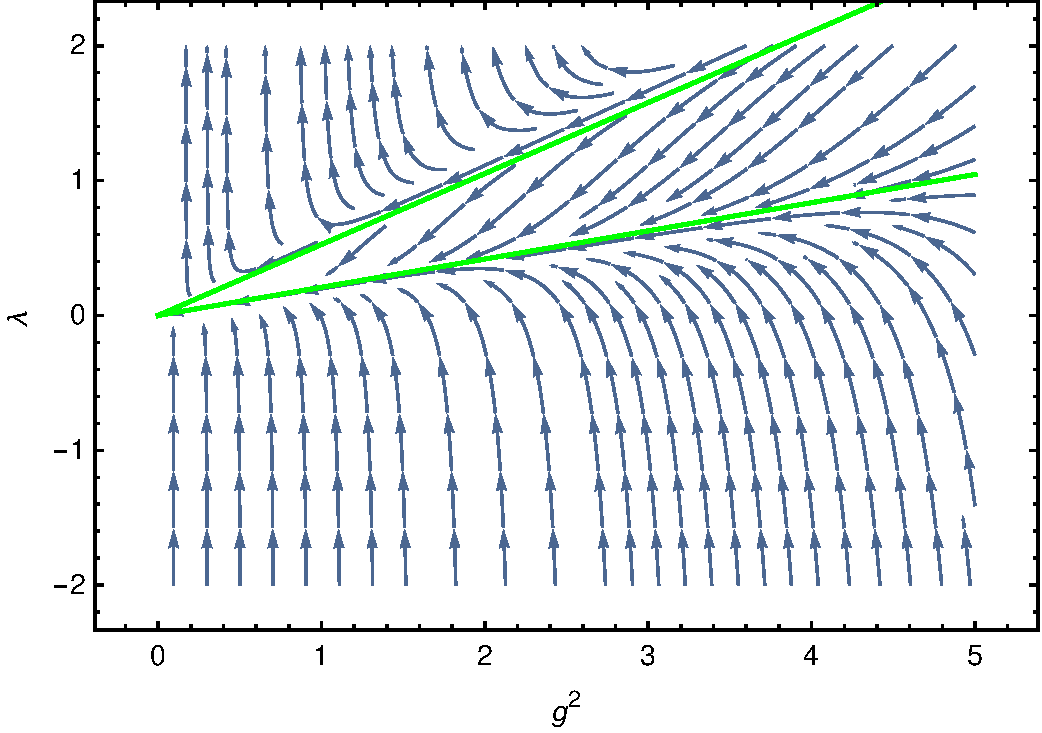
\includegraphics[width=9cm,clip]{pics/flow}
   \caption{Running of the squared gauge coupling $g^2$ and of the scalar quartic coupling $\lambda$ for a theory with SU(5) gauge group, $N_f=26$ fundamental fermions and $N_S =1$ fundamental scalars. The arrows indicate the direction of increasing energy. The green lines represent the fixed flow solutions of the renormalisation group equations, characterised by a constant ratio $\lambda/g^2$. This picture has already been published in \cite{Hansen:2017mrt}.}
  \label{flow_2D}
\end{figure}

\begin{table}[thb]
  \small
  \centering
  \caption{For different values of N, ranges in $N_f$ such that there exist completely asymptotically free solutions, in a theory with SU(N) gauge group, $N_f$ fundamental fermions and $N_S=1$ fundamental scalars.}
  \begin{tabular}{lll}\toprule
  $N$ & $N_f$  \\\midrule
  2 & No solutions \\
  3 & $15.93 < N_f < 16.25$ \\ 
  4 & 1$9.8 < N_f < 21.75$ \\
  5 & $23.56 < N_f < 27.25$ \\
  6 & $27.27 < N_f  < 32.75$ \\
  7 & $30.94 < N_f  < 38.25$ \\
  8 & $34.6 < N_f  < 43.75$ \\
  9 & $38.24 < N_f < 49.25$ \\
  10 & $41.88 < N_f < 54.75$ \\\bottomrule
  \end{tabular}
  \label{asympt_freedom}
\end{table}

\begin{figure}[thb] 
  \centering
  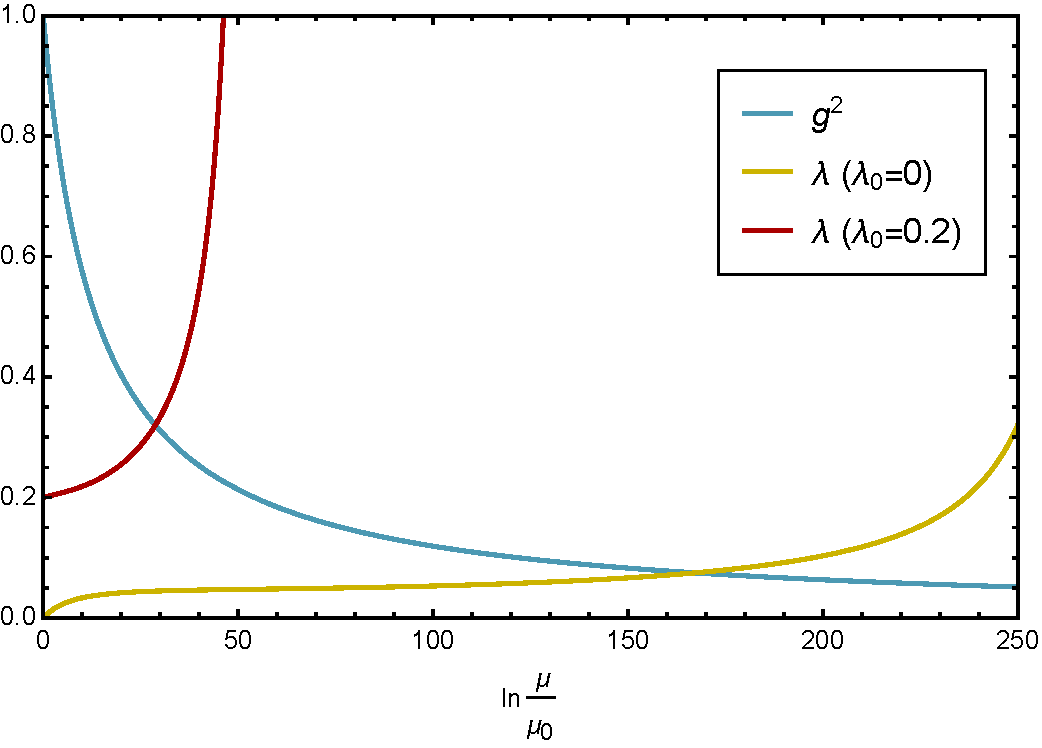
\includegraphics[width=9cm,clip]{pics/flow_N2}
  \caption{ Running of $g^2$ and $\lambda$ as functions of $\ln (\mu/\mu_0)$ in an SU(2) gauge theory with $N_f=2$ fundamental fermions and $N_S=1$ fundamental scalars. $\lambda$ is plotted for two different initial conditions: $\lambda_0 = \lambda(\mu_0) = 0$, and $\lambda_0=\lambda(\mu_0)=0.2$. This picture has already been published in \cite{Hansen:2017mrt}.}
  \label{flow_SU2}
\end{figure}

One more comment must be made regarding the case $N=2$. As previously pointed out, the fundamental representation of SU(2) is pseudo-real. One may wonder whether in this case there exist more quartic operators than the ones listed in equation \ref{quartic_operators}. It is shown in appendix \ref{app_quartic_potential} that, also in the case of an SU(2) gauge group, the most general quartic potential takes the form \ref{quartic_potential}.

%%%%%%%%%%%%%%%%%%%%%%%%%%%%%%%%%%%%%%%%%%%%%%%%%%%%%%

\section{Lattice setup}


We now move to the lattice study of the SU(2) gauge theory with two fundamental fermions and one fundamental scalar. In section \ref{running_lambda}, we discussed the running of the scalar quartic coupling, and we concluded that the SU(2) theory is not well defined at high energies because the quartic coupling diverges. Because of this, it is impossible to define the continuum limit of the lattice theory. In fact, due to the universality of the first two coefficients of the beta function, the running of the lattice bare couplings as functions of the lattice spacing is the same as shown in figure \ref{flow_SU2}, with $\mu \propto 1/a$. It follows that, at least in the region where perturbation theory is valid, there is no critical point in the space of bare lattice parameters, and the program of taking the lattice spacing to zero while moving on lines of constant physics cannot be undertaken. Instead, one can take the lattice spacing down to some small but finite value, and match the lattice theory to an effective theory with an ultraviolet cutoff. Given the running of the scalar quartic coupling shown in figure \ref{flow_SU2}, we expect the lattice theory to present a good scaling window when changing the lattice spacing, so that valuable input for phenomenological models can be provided.

For our lattice study, we generated gauge and scalar field configurations with the HiRep code, first introduced in \cite{DelDebbio:2008zf}, which we extended in order to simulate the scalar field in addition to gauge and fermions. In the following we describe the lattice action and the resulting forces needed for the implementation of the Hybrid Monte Carlo algorithm.


\subsection{Action}

For the gauge and fermion action we use the Wilson discretisation, as defined in equation \ref{lattice_action_psf}. For simplicity, we fix the lattice spacing to one, and we use the standard notation $\beta = 2 N/ g^2 = 4/g^2$. As for the scalar field $S$, we consider the Euclidean continuum action:

\begin{equation}
S_S^{cont} [A,S^{\dagger},S]= \int d^4x \biggl( (D_{\mu} S)^{\dagger} D_{\mu}S + m_S^2 |S|^ 2 + \lambda |S|^4 \biggr) \; ,
\end{equation}
%
and we discretise it by assigning 

\begin{equation}
\int \dx (D_{\mu} S)^{\dagger} D_{\mu}S \to - \sum_{x,\mu} S^{\dagger} \nabla_{\mu}^* \nabla_{\mu} S \; ,
\end{equation}
%
where

\begin{equation}
\begin{split}
&\nabla_{\mu} S(x) = U_{\mu}(x)S(x + \hat\mu) - S(x)  \\
&\nabla_{\mu}^* S(x) = S(x) - U_{\mu}(x- \hat \mu)^{\dagger} S(x- \hat \mu) \; .
\end{split}
\end{equation}
%
The resulting discretised action is: 

\begin{equation}
\begin{split}
S_S[U,S^{\dagger},S] = & \sum_x \biggl[ - \sum_{\mu} \biggl( S^{\dagger}(x) U_{\mu}(x) S(x+\hat\mu) + S^{\dagger}(x) U_{\mu}(x-\hat\mu)^{\dagger} S(x-\hat\mu) \biggr) +  \\
 & M^2 S^{\dagger}(x) S(x) + \lambda \bigl(S^{\dagger}(x) S(x) \bigr)^2 \biggr] \: ,
\end{split}
\label{scalar_lattice_action}
\end{equation}
%
where $M^2=m_S^2+8$. For future purposes, we write the action of our lattice model as:

\begin{equation}
S[U,\phi^{\dagger},\phi,S^{\dagger},S] = S_G[U] + S_F[U,\phi^{\dagger},\phi] + S_S[U,S^{\dagger},S] \: ,
\label{action}
\end{equation}
%
where $S_S$ is the scalar contribution given by equation \ref{scalar_lattice_action}, $S_G$ is the gauge contribution:

\begin{equation}
S_G[U] =  \beta \sum_{x \in \Lambda}  \sum_{\mu < \nu} \biggr[  1 - \frac{1}{\mathrm{N}} \re \tr  [U_{\mu \nu}] \biggl ] \: ,
\end{equation}
%
and $S_F$ the pseudofermion contribution (for two mass-degenerate fermion flavours):

\begin{equation}
S_F[U,\phi^{\dagger},\phi]  = \sum_{x,y \in \Lambda} \phi^{\dagger}(x) Q^{-2}(x \vert y)\phi(y) \equiv \phi^{\dagger} Q^{-2} \phi \: ,
\end{equation}
%
where we introduced a short-hand notation that will be useful in the following.


\subsection{Forces}
\label{Forces}

In order to implement the Hybrid Monte Carlo algorithm, we introduce the Hamiltonian:

\begin{equation}
H = \frac{1}{2} T_R\sum_{x,\mu}\sum_{a=1}^{N^2-1} \pi_a (x, \mu)^2 + \sum_x \sum_{i=1}^N P_i(x)P^*_i(x) + S[U,\phi^{\dagger},\phi,S^{\dagger},S] \: ,
\end{equation}
%
where $\pi_a(x,\mu)$ and $P_i(x)$ are the momenta associated to the gauge and scalar fields, and $S$ is the action \ref{action}. Here, to be more general, we are referring to an SU(N) gauge group. $T_R$ is the normalisation of the SU(N) generators in the representation $R$, defined by: $\mathrm{tr} (T^aT^b) = T_R \delta^{ab}$.
In this setup, only gauge and scalar fields evolve dynamically along the molecular dynamics trajectory. The pseudofermions are updated before starting every new trajectory according to the following rule: a field $\chi$ is extracted out of a Gaussian distribution, with probability $P[\chi] \propto \exp [-\chi^{\dagger} \chi]$, and then the pseudofermion field is defined as: $\phi = D \chi$, where $D$ is the Wilson-Dirac operator \ref{Wilson-Dirac}. The field $\phi$ defined in this way is correctly distributed according to:


\begin{equation}
\det[Q^2] = \det[D]^2 = \det[DD^{\dagger}] = \pi^{-N} \int \prod_{x \in \Lambda} \mathrm{d} \phi(x) \mathrm{d} \phi^{\dagger}(x) \exp \bigl[ 
-\phi^{\dagger}(DD^{\dagger})^{-1}  \phi \bigr] \: .
\end{equation}
%
We express the link variables as:
\begin{equation}
U_{\mu}(x)=\exp [\frac{i}{T_R} q_a(x,\mu) T^a] \: , 
\end{equation}
%
and we assign the conjugate momenta as follows:

\begin{equation}
\begin{split}
& q_a(x,\mu) \to \pi_a(x,\mu) \\
& S_i(x) \to P_i(x) \; .
\end{split}
\end{equation}
%
Hamilton's equations are given by:

\begin{equation}
\begin{split}
& \dot{q}_a(x,\mu) = \frac{\partial H}{\partial \pi_a(x,\mu)}  =T_R \pi_a(x,\mu) \\
& \dot{\pi}_a(x,\mu) = -\frac{\partial H}{\partial q_a(x,\mu)} = -\frac{\partial S_G}{\partial q_a(x,\mu)} -\frac{\partial S_F}{\partial q_a(x,\mu)} -\frac{\partial S_S}{\partial q_a(x,\mu)} \\
& \dot{S}_i(x) = \frac{\partial H}{\partial P_i(x)} = P^*_i(x) \\
& \dot{P}_i(x) =  -\frac{\partial H}{\partial S_i(x)} = -\frac{\partial S_S}{\partial S_i(x)}  \: ,\\ 
\end{split} 
\label{hamilton}
\end{equation} 
%
where the dot indicates the derivative with respect to molecular dynamics time. For brevity we omitted the equations for $\dot S^*$ and $\dot P^*$, which are simply given by the complex conjugate of the last two lines in \ref{hamilton}.
The first line of \ref{hamilton} can be rewritten in terms of the link variables as follows:


\begin{equation}
\dot{U_{\mu}}(x)= i \pi_a(x,\mu)T^a U_{\mu}(x) \; .
\end{equation}
%
The driving forces are given by:

\begin{equation}
\bullet \qquad \frac{\partial S_G}{\partial q_a(x,\mu)} = - \frac{\beta}{N} \frac{1}{T_R} \mathrm{Re \; tr} \biggl[ i T^a U_{\mu}(x) V^{\dagger}_{\mu} (x) \biggr]
\end{equation}
%
where $V_{\mu}(x) = \sum_{\nu \neq \mu} \bigl[ U_{\nu}(x) U_{\mu}(x+\hat\nu) U_{\nu}^{\dagger}(x+\hat\mu) + 
U_{\nu}^{\dagger}(x - \hat\nu) U_{\mu}(x - \hat\nu) U_{\nu}(x-\hat\nu+\hat\mu)\bigr]$ is the sum of the staples around the link $U_{\mu}(x)$,


\begin{equation}
\bullet \qquad\frac{\partial S_F}{\partial q_a(x,\mu)} =   -\biggl[ \phi^{\dagger} Q^{-2}\frac{\partial Q}{\partial q_a(x,\mu)} Q^{-1} \phi + \phi^{\dagger} Q^{-1} \frac{\partial Q}{\partial q_a(x,\mu)} Q^{-2} \phi \biggr] 
\end{equation}
%
where

\begin{equation}
\frac{\partial Q(x \vert y)}{\partial q_a(z,\mu)} = \gamma_5 \biggl( -\frac{i}{2T_R} (\id - \gamma_{\mu}) T^a U_{\mu}(z) \delta_{y,z+\hat\mu} \delta_{x,z} +\frac{i}{2T_R}(\id + \gamma_{\mu}) U_{\mu}^{\dagger}(z) T^a \delta_{y,z} \delta_{x-a\hat\mu,z} \biggr) \: ,
\end{equation}


\begin{equation}
\bullet \qquad
\frac{\partial S_S}{\partial q_a(x,\mu)} = - \frac{2}{T_R} \; \mathrm{Re} \biggl[ S^{\dagger}(x) i T^a U_{\mu}(x) S(x+\hat\mu) \biggr] 
\end{equation}



\begin{equation}
\begin{split}
\bullet \qquad
\frac{\partial S_S}{\partial S_i(x)} = & - \sum_{\mu} \biggl( S^*_k(x-\hat \mu) U_{\mu}(x-\hat\mu)_{ki} + S^*_k(x+\hat\mu) U_{\mu}(x)^{\dagger}_{ki} \biggr) +  \\
& + M^2 S_i^*(x) + 2 \lambda S_k^*(x) S_k(x) S_i^*(x) \: .
\end{split}
\end{equation}
%
Hamilton's equations \ref{hamilton} are to be solved numerically, thus generating the molecular dynamics trajectory. In this work we used a second-order Omelyan integrator \cite{PhysRevE.65.056706,OMELYAN2003272} for the numerical integration.


%%%%%%%%%%%%%%%%%%%%%%%%%%%%%%%%%%%%%%%%%%%%%%%%%%%%%%


\section{Spectrum}


\subsection{Mesons}

In this section, we present our results on the meson spectrum of the SU(2) gauge theory with two fundamental fermions and one fundamental scalar. We measured the mass of the isospin-triplet pseudoscalar ($m_{PS}$) and vector ($m_V$) mesons. The interpolating operators for these observables are defined in section \ref{meson_masses}. We also measured the fermion mass $m_{PCAC}$ via the PCAC relation, as described in section \ref{measure_PCAC}. Moreover, we measured the Goldstone boson decay constant $f_{PS}$. This observable (once renormalised) can be used to express the lattice spacing in physical units. In fact, as discussed in section \ref{SU2_composite_Higgs}, the $W$ boson mass is given by\footnote{Here we use a different normalisation for the Goldstone boson decay constant with respect to section \ref{SU2_composite_Higgs}. The two conventions are related by: $f = f_{PS}/(2 \sqrt 2)$.}:

\begin{equation}
m_W = \frac{g_{EW}}{2} (f_{PS})^{ren}_0 \sin \theta \: ,
\end{equation}
%
where $g_{EW}$ is the SU(2)$_L$ electroweak gauge coupling and $\theta$ the alignment angle. $(f_{PS})^{ren}_0$ denotes the renormalised Goldstone boson decay constant in the chiral limit ($m_{PCAC} \to 0$). It follows that the experimental value of $m_W$ is recovered by fixing $(f_{PS})^{ren}_0 \sin \theta = v$, $v = 246 \: \mathrm{GeV}$ being the Higgs vacuum expectation value. $f_{PS}$ is computed as:

\begin{equation}
f_{PS} = \frac{2 m_{PCAC}}{m_{PS}^2} G_{PS} \: ,
\end{equation}
%
where $G_{PS}$ is obtained from the large-t behaviour of the correlator $C_{\gamma_5}(t)$, defined in section \ref{meson_masses}:

\begin{equation}
C_{\gamma_5}(t) \underset{t \to \infty}{\sim} -\frac{G^2_{PS}}{m_{PS}} e^{-m_{PS} t} \: .
\end{equation}


Renormalisation has not been addressed in our work yet, and the values of $m_{PCAC}$ and $f_{PS}$ that we quote are unrenormalised. Moreover, all our results, listed in table \ref{data}, are expressed in lattice units. For our measurements, we chose values of the inverse gauge coupling $\beta$ and of the bare fermion mass $m_f$ that have already been studied in the SU(2) gauge theory with two fundamental fermions \cite{Arthur:2016dir}. In particular, at the current status of our analysis, we considered one single value of $\beta$ ($\beta = 2$) and two values of the bare fermion mass: $m_f = -0.94, -0.952$. For each choice of $m_f$, we simulated several values of the squared scalar mass $m_S^2$, and, in the case of $m_f = -0.94$, we repeated the analysis for two different values of the scalar quartic coupling $\lambda$. In a few cases, we repeated the measurements with the same bare parameters at two different lattice volumes. We consider lattices with the same extent in all spacial directions $L_1 = L_2 = L_3 \equiv L$, and we denote the lattice time extent by $T \equiv L_0$. 

Since we will use quite often the SU(2) theory with two fundamental fermions as a comparison, we will shortly refer to it as the SU(2)-2F model, and we will make reference to the most recent results published in \cite{Arthur:2016dir}.
In figure \ref{mesons_mS}, we plot the PCAC mass, the meson masses and the Goldstone boson decay constant as functions of the squared scalar mass $m_S^2$. Together with our data points, we report the results for the same observables obtained in the SU(2)-2F model (dashed lines).  We observe that, provided $m_S^2$ is large enough, the results of the SU(2)-2F model are recovered, while for $m_S^2 \lesssim 1$ deviations from those results can be observed in all the considered observables. Moreover, for $\lambda = 2$ and $m_f = -0.94$, we observe a sharp change of behaviour around $m_S^2 \simeq -3.2$, presumably corresponding to a phase transition. In particular, at ($m_f$, $\lambda$, $m_S^2$) = (-0.94, 2, -3.6), the PCAC mass is negative, $m_{PS}$ and $m_V$ are almost degenerate and $f_{PS}$ is compatible with zero. For $m_f = -0.94$, $\lambda = 2$ and $m_S^2 \leq -3.2$, the simulations become significantly more time-consuming than for larger values of $m_S^2$, and require a very fine integration step in the molecular dynamics trajectories. In the case of $m_f = -0.94$ and $\lambda = 0$, we were not able to run simulations at $m_S^2 < -1$. We believe that this is due to instability of the scalar potential. It will be shown in the next section that a similar situation occurs in the SU(2) model with one fundamental scalar and no fermions (SU(2)-Higgs model).



\begin{figure}[thb] 
\begin{adjustwidth}{-4em}{-4em}
  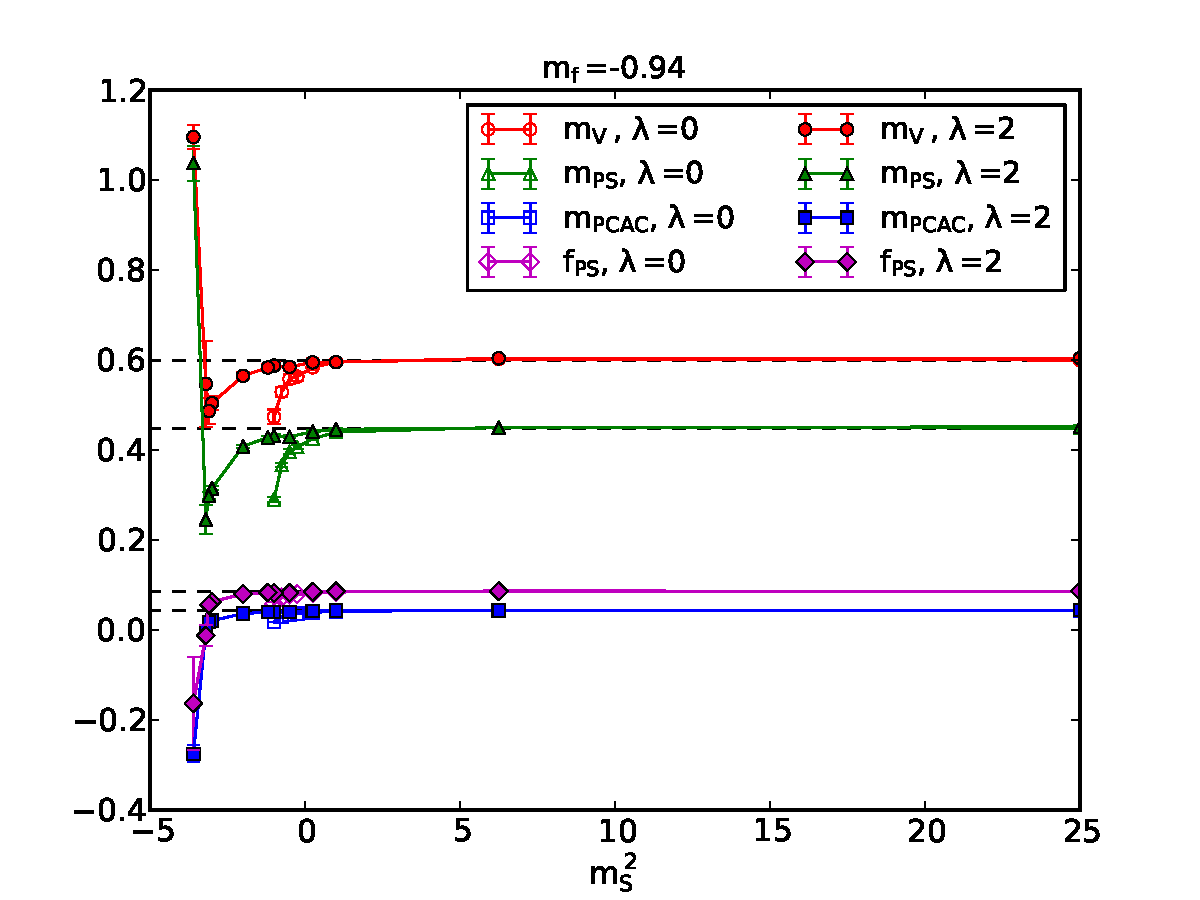
\includegraphics[width=9cm,clip]{pics/mesons_094} ~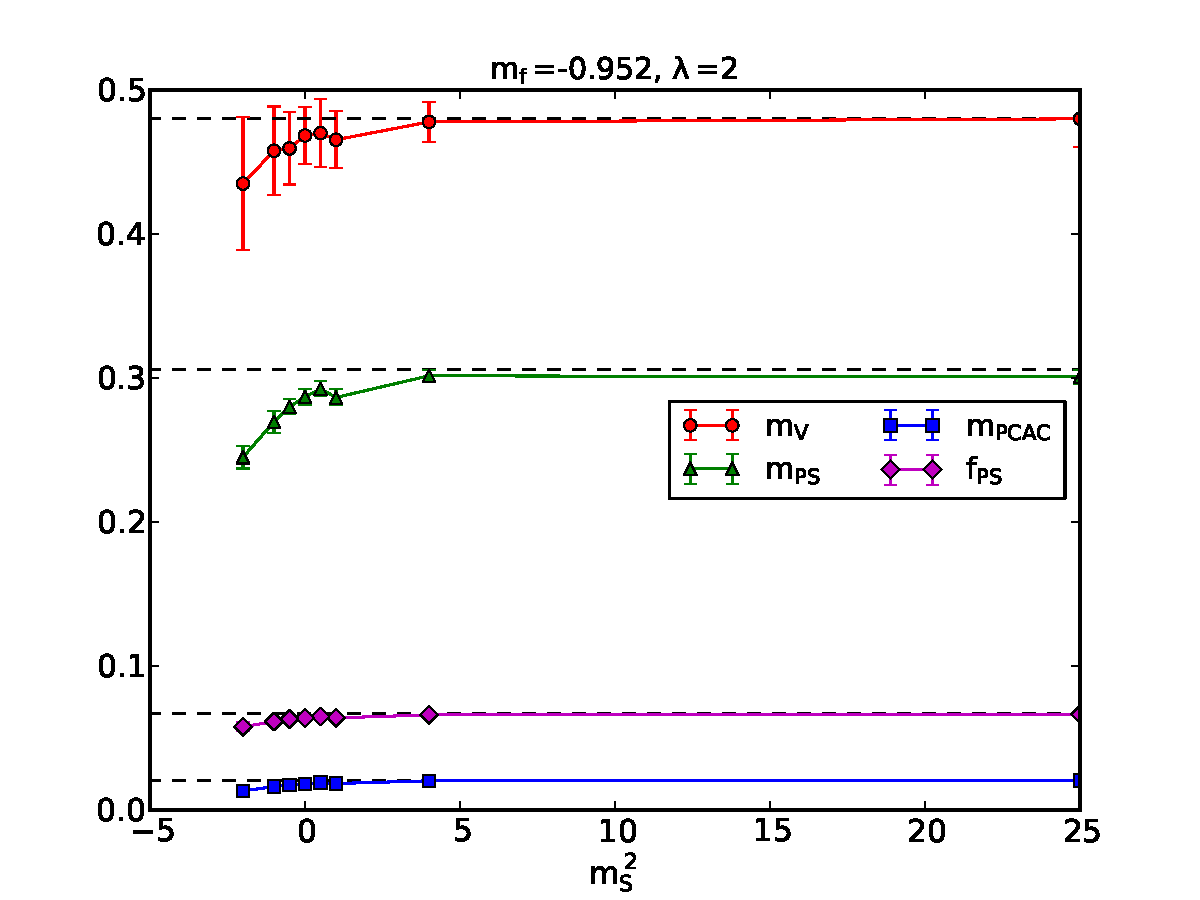
\includegraphics[width=9cm,clip]{pics/mesons_0952} 
  \end{adjustwidth}
  \caption{Fermion mass ($m_{PCAC}$), pseudoscalar meson mass ($m_{PS}$), vector meson mass ($m_V$) and Goldstone boson decay constant ($f_{PS}$) as functions of the squared scalar mass $m_S^2$. Together with our data points, we report the results for the same observables obtained in the SU2-2F model (dashed lines). In the left panel we plot the results for $m_f = -0.94$ and two different values of $\lambda$, while in the right panel there appear the results for $m_f = -0.952$ and $\lambda = 2$.}
  \label{mesons_mS}
\end{figure}

In figure \ref{mesons_094_PCAC}, we plot $m_{PS}$, $m_V$ and $f_{PS}$ as functions of $m_{PCAC}$, for $m_f = -0.94$. In the left panel we report all our data points, while in the right panel we omit two points, corresponding to ($\lambda$, $m_S^2$) = (2, -3.6), (2, -3.2). Together with our data, we report fits to the data of the SU(2)-2F model. The forms of the fitting functions for $m_{PS}$ and $f_{PS}$ are motivated by chiral perturbation theory, and are given by:

\begin{equation}
\frac{m_{PS}^2}{m_{PCAC}} = M_0 \bigl[ 1 + M_1 m_{PCAC} \log (m_{PCAC}) + M_2 m_{PCAC} \bigr] \: ,
\label{fit_PS}
\end{equation}

\begin{equation}
f_{PS} = F_0 \bigl[ 1+ F_1 m_{PCAC} \log (m_{PCAC}) + F_2 m_{PCAC} \bigr] \: ,
\label{fit_fPS}
\end{equation}
%
while for $m_V$ the following polynomial ansatz is used:

\begin{equation}
m_V = V_0 + V_1 m_{PCAC} + V_2 m_{PCAC}^2 \: .
\label{fit_V}
\end{equation}
%
It can be observed that, once the points ($\lambda$, $m_S^2$) = (2, -3.6), (2, -3.2) are excluded, there is very good agreement between our data and the fits in the SU(2)-2F model. We stress the fact that the curves in figure \ref{mesons_094_PCAC} are obtained in the SU(2)-2F model by fitting data at fixed $\beta$ and varying $m_f$, while our data points shown in the figure are obtained at fixed $\beta$ and $m_f$, and varying $m_S^2$, for two different values of $\lambda$. In the right panel of figure \ref{mesons_094_PCAC}, the black points represent measurements obtained in larger lattice volumes. It can be observed from the data in table \ref{data}, that large finite volume corrections in the PCAC mass and pseudoscalar meson mass occur at ($m_f$, $\lambda$, $m_S^2$) = (-0.94, 0, -1). The same effect is not observed at ($m_f$, $\lambda$, $m_S^2$) = (-0.94, 0, 0.0625), where we also repeated the measurements in two different volumes. 


\begin{figure}[thb] 
\begin{adjustwidth}{-4em}{-4em}
  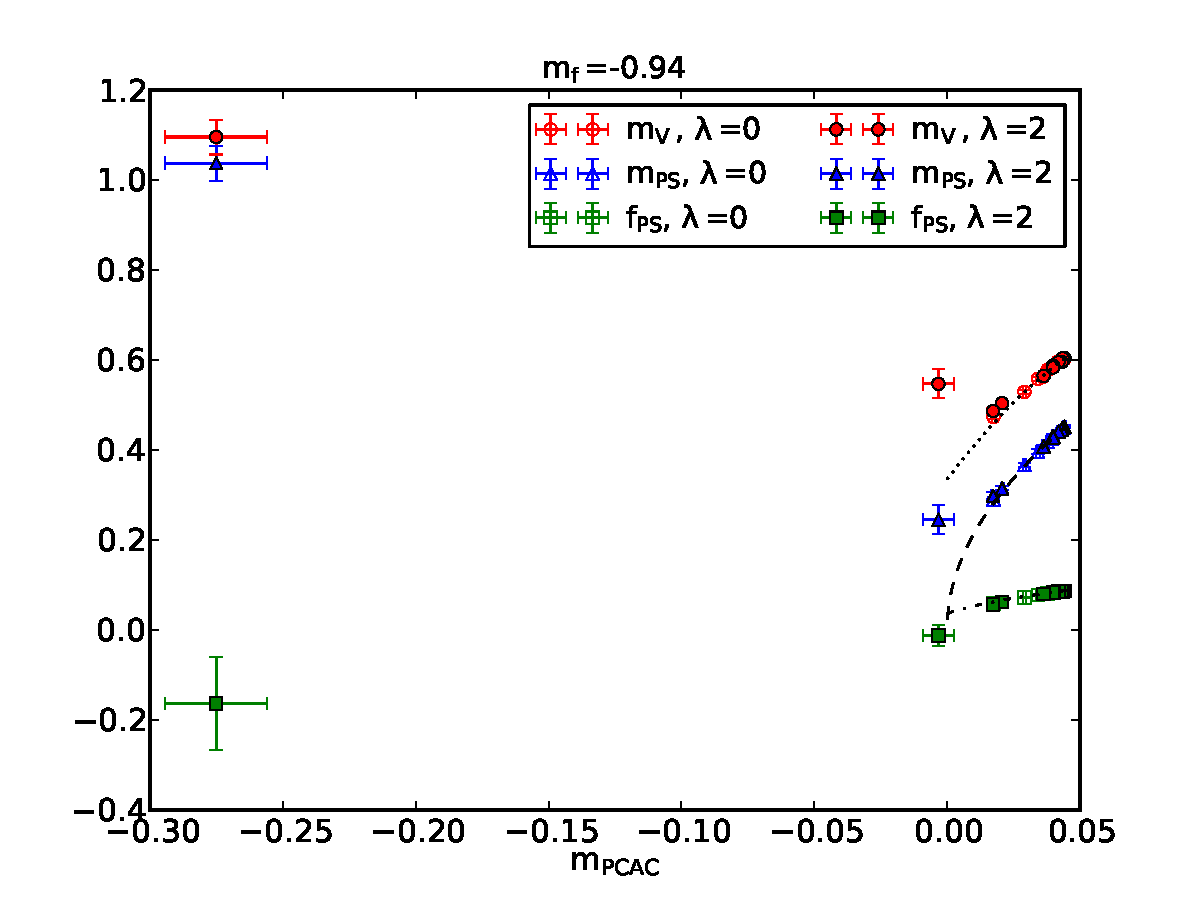
\includegraphics[width=9cm,clip]{pics/mesons_094_PCAC} ~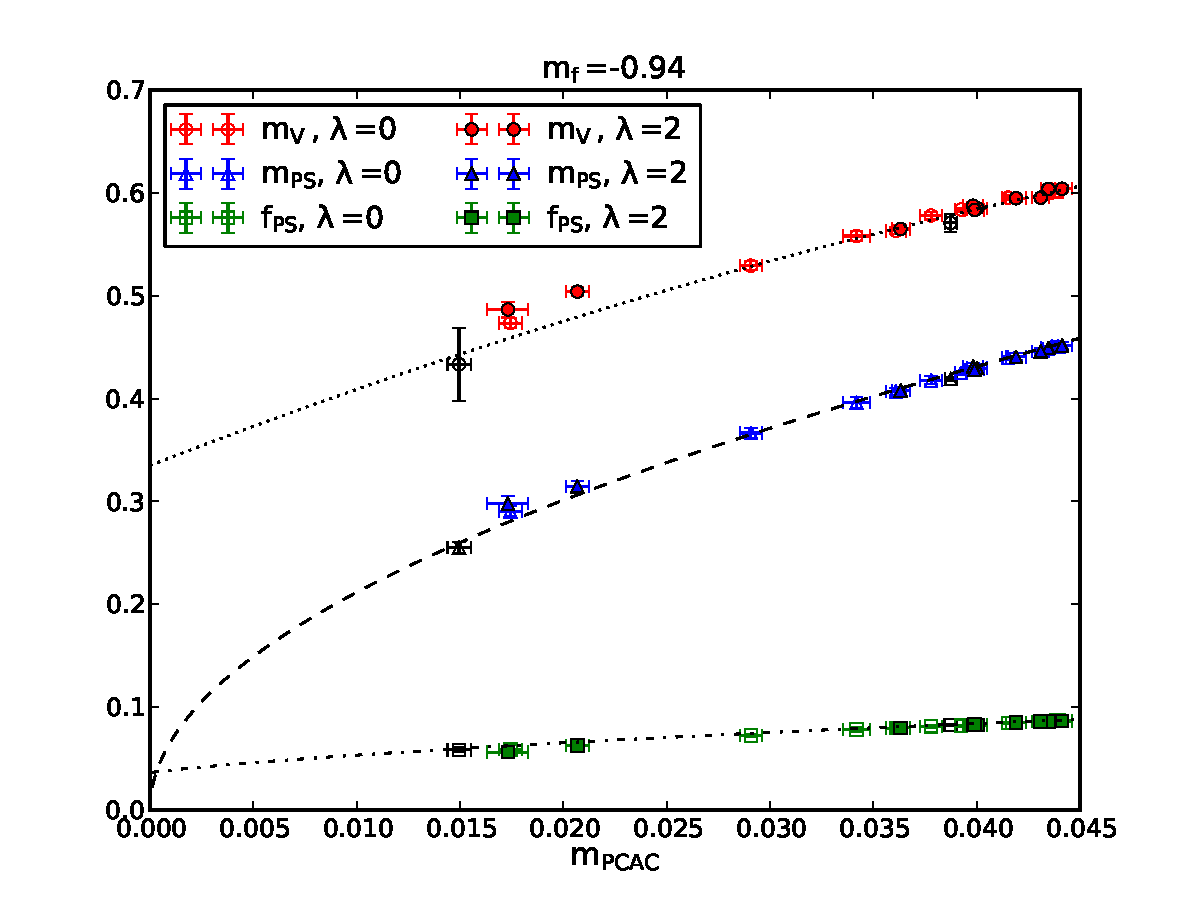
\includegraphics[width=9cm,clip]{pics/mesons_094_PCAC_fit}
   \end{adjustwidth}
  \caption{Pseudoscalar meson mass ($m_{PS}$), vector meson mass ($m_V$) and Goldstone boson decay constant ($f_{PS}$) as functions of $m_{PCAC}$, at $m_f = -0.94$. In the left panel all the available data are included, while in the right panel we excluded the points ($\lambda$, $m_S^2$) = (2, -3.6), (2, -3.2). The dotted, dashed and dash-dotted lines are fits to the data of the SU(2)-2F model, obtained by fitting data at fixed $\beta = 2$ and varying $m_f$, by using the functional forms \ref{fit_V}, \ref{fit_PS}, \ref{fit_fPS}. The black data points in the right panel represent measurements obtained in a larger volume $L=24$, $T=48$. All the other points correspond to $L=16$, $T=32$.}
  \label{mesons_094_PCAC} 
\end{figure}


In figure \ref{mesons_l2_PCAC} we plot $m_{PS}$, $m_V$ and $f_{PS}$ as functions of $m_{PCAC}$, for $\lambda = 2$ and the two available values of $m_f$. The points ($m_f$, $\lambda$, $m_S^2$) = (-0.94, 2, -3.6), (-0.94, 2, -3.2) are excluded. The curves are the same as in figure \ref{mesons_094_PCAC}. We again observe an impressive agreement with the data of the SU(2)-2F model. As the PCAC mass becomes lighter, the data at $m_f = -0.94$ start to show small deviations with respect to the curves, as the presumed phase transition approaches, while the $m_f = -0.952$ data are still in very good agreement with the curves. We presume that the phase transition will occur also in the case $m_f = -0.952$, $\lambda = 2$, even though we have not yet reached the critical value of $m_S^2$ in our analysis.


\begin{figure}[thb] 
\begin{center}
 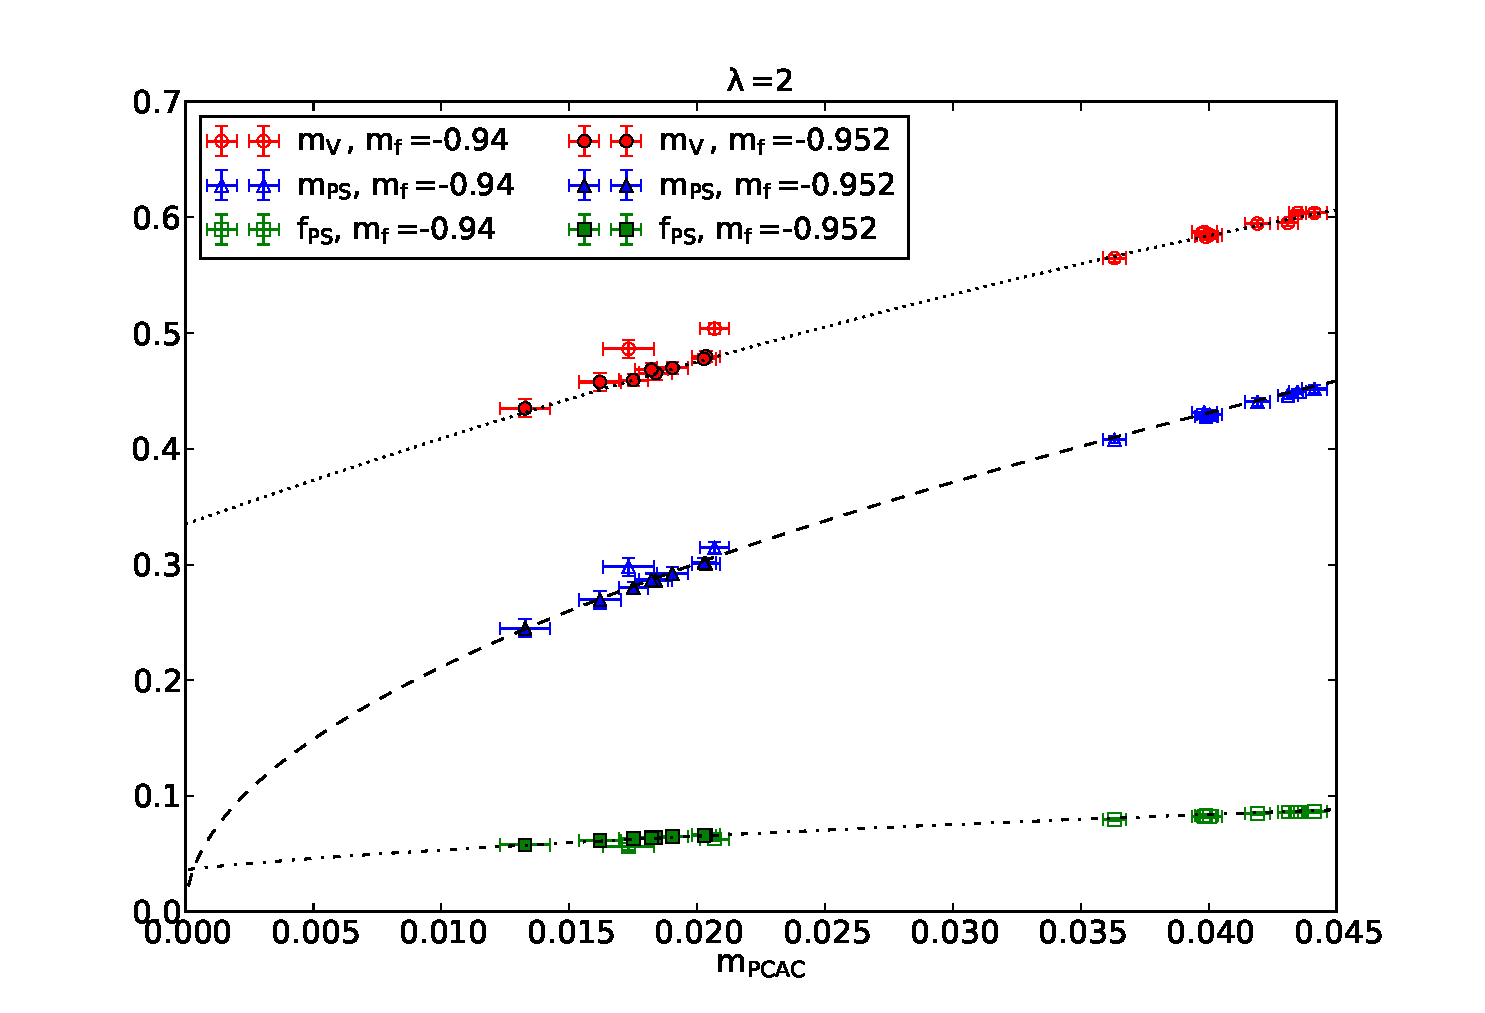
\includegraphics[width=11cm,clip]{pics/mesons_l2_PCAC_fit}
  \end{center}
  \caption{Same as the right panel of figure \ref{mesons_094_PCAC}, but for fixed $\lambda = 2$ and two different values of $m_f$.}
  \label{mesons_l2_PCAC}
\end{figure}

To conclude, our somewhat preliminary analysis of the meson spectrum of the SU(2) gauge theory with two fundamental fermions and one fundamental scalar already shows some interesting results. First of all, there seems to exist a phase with broken fermion-flavour symmetry, with Goldstone boson states (the pseudoscalar mesons) whose mass goes to zero in the limit of vanishing $m_{PCAC}$ and whose decay constant remains finite in the same limit. This seems to indicate that additional scalar fields may not dramatically affect the symmetry breaking pattern of a gauge-fermion theory, and it is encouraging from the point of view of composite Higgs models based on the fundamental partial compositeness paradigm. However, we found two kinds of obstacles in moving towards small values of the PCAC mass: at $m_f = -0.94$, $\lambda = 0$, we found a critical value of the squared scalar mass, $m_S^2 = -1$, below which the simulations do not work, due presumably to instability of the scalar potential (we will discuss this point in more detail in the next section). At $m_f = -0.94$, $\lambda = 2$, we observed an abrupt change of behaviour of the meson observables around $m_S^2 = -3.2$, presumably due to a phase transition. In particular, we find a point with zero PCAC mass and nonzero $m_{PS}$, ($m_S^2$ = -3.2) and one point with negative PCAC mass and degenerate $m_{PS}$ and $m_V$ ($m_S^2 = -3.6$). An extension of our analysis to smaller values of the bare fermion mass and larger values of $\beta$ will give us a better understanding of the phase structure of the model. 

Another interesting result is the impressive agreement between our results and the results  of the SU(2) theory with two fundamental fermions \cite{Arthur:2016dir}, once the meson masses and Goldstone boson decay constant are expressed as functions of $m_{PCAC}$. In particular, our data fall pretty accurately on top of the curves obtained by fitting the data of the SU(2)-2F model, provided we exclude some of the data which presumably belong to a different phase. This seems to indicate that the main influence of the scalar field on the meson observables is due to a shift of the PCAC mass. The last interesting observation, for which we have no explanation at the moment, is the occurrence of large finite volume effects in $m_{PCAC}$ and $m_{PS}$ at ($m_f$, $\lambda$, $m_S^2$) = (-0.94, 0, -1).


\begin{table}
\begin{adjustwidth}{-4em}{-4em}
\begin{tabular}{l  l l l l l l l l l l}
\toprule
$m_f$ & $\lambda$ & $m_S^2$ & $L$ & $T$ & $m_{PCAC}$ & $m_{PS}$ & $f_{PS}$ & $m_V$ & $\mathcal Q_L$ & $\mathcal Q_C$ \\ 
\hhline{===========}
-0.94 & 0 & 25 & 16 & 32 & 0.0435(2) & 0.449(1) & 0.0860(6) & 0.600(3) \\
-0.94 & 0 & 6.25 & 16 & 32 & 0.0439(2) & 0.450(1) & 0.0868(7) & 0.602(2) & 2.03(3) $\times 10^{-6}$ & 0.1626(7)\\
-0.94 & 0 & 1 & 16 & 32 & 0.0415(3) & 0.440(2) & 0.084(1) & 0.595(5)\\
-0.94 & 0 & 0.25 & 16 & 32 & 0.0392(3) & 0.425(2) & 0.082(1) & 0.584(5) \\
-0.94 & 0 & 0.0625 & 16 & 32 & 0.0385(4) & 0.420(3) & 0.082(1) & 0.571(8) & 1.15(2) $\times 10^{-5}$ & 0.174(2)\\
-0.94 & 0 & 0.0625 & 24 & 48 & 0.0387(3) & 0.419(2) & 0.083(1) & 0.57(1) &  2.24(5) $\times 10^{-6}$ & 0.0729(3)\\
-0.94 & 0 & 0 & 16 & 32 & 0.0378(6) & 0.418(4) & 0.081(2) & 0.578(8)\\
-0.94 & 0 & -0.25 & 16 & 32 & 0.0361(5) & 0.407(3) & 0.080(1) & 0.56(1)\\
-0.94 & 0 & -0.5 & 16 & 32 & 0.0342(6) & 0.396(5) & 0.078(2) & 0.56(1)\\
-0.94 & 0 & -0.75 & 16 & 32 & 0.0291(5) & 0.367(4) & 0.073(2) & 0.53(1)\\
-0.94 & 0 & -1 & 16 & 32 & 0.0174(6) & 0.290(5) & 0.059(4) & 0.47(2) & 1.01(4) $\times 10^{-4}$ & 0.233(2)\\
-0.94 & 0 & -1 & 24 & 48 & 0.0150(6) & 0.255(5) & 0.058(2) & 0.43(4) & 2.0(1) $\times 10^{-5}$ & 0.117(1)\\
\midrule
-0.94 & 2 & 25 & 16 & 32 & 0.0441(5) & 0.452(3) & 0.087(1) & 0.604(8)\\
-0.94 & 2 & 6.25 & 16 & 32 & 0.0435(3) & 0.449(2) & 0.086(1) & 0.604(6)\\
-0.94 & 2 & 1 & 16 & 32 & 0.0431(4) & 0.446(3) & 0.086(1) & 0.595(7)\\
-0.94 & 2 & 0.25 & 16 & 32 & 0.0419(5) & 0.441(3) & 0.085(1) & 0.60(1) \\
-0.94 & 2 & -0.5 & 16 & 32 & 0.0400(5) & 0.430(4) & 0.082(2) & 0.59(1)\\
-0.94 & 2 & -1 & 16 & 32 & 0.0398(5) & 0.431(3) & 0.082(2) & 0.59(1)\\
-0.94 & 2 & -1.2 & 16 & 32 & 0.0399(4) & 0.428(3) & 0.083(1) & 0.583(8)\\
-0.94 & 2 & -2 & 16 & 32 & 0.0363(4) & 0.408(3) & 0.080(1) & 0.565(8)\\
-0.94 & 2 & -3 & 16 & 32 & 0.0207(6) & 0.315(5) & 0.063(2) & 0.50(1)\\
-0.94 & 2 & -3.1 & 16 & 32 & 0.017(1) & 0.298(8) & 0.056(3) & 0.49(3) & 1.02(3) $\times 10^{-4}$ & 0.233(4)\\
-0.94 & 2 & -3.2 & 16 & 32 & -0.003(6) & 0.25(3) & -0.01(2) & 0.5(1) & 3.8(7) $\times 10^{-4}$ & 0.34(2)\\
-0.94 & 2 & -3.6 & 16 & 32 & -0.28(2) & 1.04(4) & -0.2(1) & 1.10(3) & 0.2166(1) & 1.0965(3)\\
\midrule
-0.952 & 2 & 25 & 32 & 32 & 0.0203(5) & 0.301(5) & 0.066(2) & 0.48(2) & 7.1(2) $\times 10^{-8}$ & 0.0472(3)\\
-0.952 & 2 & 4 & 32 & 32 & 0.0203(5) & 0.302(4) & 0.066(1) & 0.48(1) & 3.07(5) $\times 10^{-7}$ & 0.0466(3)\\
-0.952 & 2 & 1 & 32 & 32 & 0.0184(6) & 0.286(6) & 0.064(2) & 0.47(2) & 5.4(1) $\times 10^{-7}$ & 0.0486(3)\\
-0.952 & 2 & 0.5 & 32 & 32 & 0.0190(6) & 0.292(5) & 0.065(2) & 0.47(2) & 6.1(1) $\times 10^{-7}$ & 0.0480(3) \\
-0.952 & 2 & 0 & 32 & 32 & 0.0182(7) & 0.287(5) & 0.064(2) & 0.47(2) &  7.1(2) $\times 10^{-7}$ & 0.0486(4)\\
-0.952 & 2 & -0.5 & 32 & 32 & 0.0175(6) & 0.280(5) & 0.063(2) & 0.46(3) & 8.9(2) $\times 10^{-7}$ & 0.0501(4)\\
-0.952 & 2 & -1 & 32 & 32 & 0.0162(8) & 0.270(8) & 0.061(3) & 0.46(3) & 1.10(3) $\times 10^{-6}$ & 0.0509(6)\\
-0.952 & 2 & -2 & 32 & 32  & 0.013(1) & 0.245(8) & 0.058(3) & 0.43(5) & 1.8(2) $\times 10^{-6}$ & 0.0560(7)\\
\bottomrule
\end{tabular}
\end{adjustwidth}
\caption{In this table we report our results, obtained at a fixed value of the inverse gauge coupling $\beta = 2$, and different values of $m_f$, $\lambda$ and $m_S^2$. The observables under analysis are: the fermion mass $m_{PCAC}$, the pseudoscalar meson mass $m_{PS}$, the vector meson mass $m_V$, the Goldstone boson decay constant $f_{PS}$ and the gauge-dependent order parameters $\mathcal Q_L$ and $\mathcal Q_C$. The latter have only been measured in some of the ensembles. All the results are expressed in lattice units. The values of $m_{PCAC}$ and $f_{PS}$ are unrenormalised.}
\label{data}
\end{table}



\subsection{Bound states with the scalar}




%%%%%%%%%%%%%%%%%%%%%%%%%%%%%%%%%%%%%%%%%%%%%%%%%%%%%%

\section{Higgs phase}

In this section we address the question of whether the scalar field can induce spontaneous breaking of the gauge symmetry in our model. We take inspiration from \cite{Caudy:2007sf}, where the phase diagram of the SU(2)-Higgs model is analysed in relation to the question of spontaneous gauge symmetry breaking. In studies of the SU(2)-Higgs model, the scalar field action is usually expressed as:

\begin{equation}
S_S =  \sum_x \biggl[ S^{\dagger}(x) S(x) + \tilde \lambda \bigl( S^{\dagger}(x) S(x) - 1 \bigr)^2 
 - \gamma\sum_{\mu}   \biggl( S^{\dagger}(x) U_{\mu}(x) S(x+\hat\mu) +  S^{\dagger}(x) U_{\mu}(x-\hat\mu)^{\dagger} S(x-\hat\mu)\biggr)  \biggr] \; ,
\end{equation}
%
where the coefficients $\tilde \lambda$ and $\gamma$ are related to our $\lambda$ and $m_S^2$ by the following equations:

\begin{equation}
\begin{cases}
\lambda = \tilde \lambda/\gamma^2\\
m_S^2 = (1-2\tilde\lambda)/\gamma - 8 
\end{cases} \: .
\end{equation}
%
A schematic picture of the phase diagram of the SU(2)-Higgs model, in the infinite-$\tilde \lambda$ limit, is given in the upper panel of figure \ref{SU2H_phase_diagram}. The infinite-$\tilde \lambda$ limit corresponds to a fixed-length scalar field: $S^{\dagger} S \equiv 1$. For $(\beta,\gamma) \ll 1$ the system is in a confinement-like phase, with a linear potential between static colour sources (up to a maximal distance where string breaking occurs due to the formation of scalar-antiscalar pairs) and a rich spectrum of QCD-like bound states. For $(\beta,\gamma) \gg 1$, the system is in a Higgs-like phase, with Yukawa-type potential between static sources and a spectrum of three massive vector bosons and a single scalar particle. The two phases are partially separated by a line of first order phase transitions, which terminates in the middle of the diagram. The Higgs and confinement phases are analytically connected \cite{Fradkin:1978dv,OSTERWALDER1978440}: any two points in the phase diagram can be connected by a path over which the expectation value of any local gauge-invariant observable varies analytically. Also the spectrum, which appears to be qualitatively very different in the two phases, changes smoothly along this analytical path. In \cite{Wurtz:2013ova}, the spectrum of the SU(2)-Higgs model is measured in the Higgs phase, and the observed states are found to be consistent with collections of almost noninteracting Higgs and $W$ bosons. The same gauge-invariant operators with all possible quantum numbers are to be used to measure the spectrum in both the Higgs and the confinement phase. While these operators generate hadron-like and "$W$-ball" states in the confinement phase, they correspond to weakly-interacting multi-particle states in the Higgs phase, and the transition between the two regimes occurs smoothly. 

The authors of \cite{Caudy:2007sf} address the question of whether the concept of gauge symmetry breaking can be used to distinguish between the Higgs and the confinement phase, i.e. they wonder whether the phase diagram of the SU(2)-Higgs model can be unambiguously separated in a symmetric region and a broken-symmetry region. The first thing that they point out, is that gauge symmetries cannot be spontaneously broken, due to the Elitzur theorem \cite{Elitzur:1975im}. As a consequence, unless the gauge is fixed, the vacuum expectation value of the scalar field is always zero. Only global subgroups of the gauge symmetry group can be spontaneously broken. "Global" refers to transformations depending on a finite number of parameters, which is independent of the volume. As a contrast, local transformations depend on a number of parameters which grows with the lattice volume. A global subgroup can be selected by fixing a gauge which leaves the 




\begin{figure}[thb] 
\begin{center}
  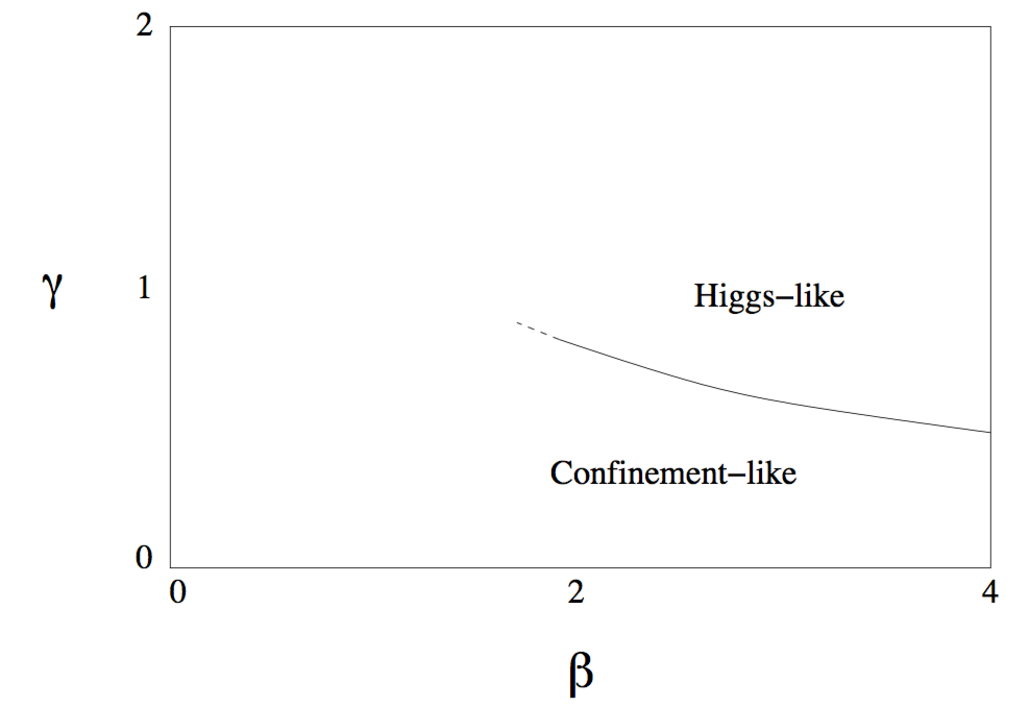
\includegraphics[width=8.8cm,clip]{pics/SU2H_phase_diagram}
  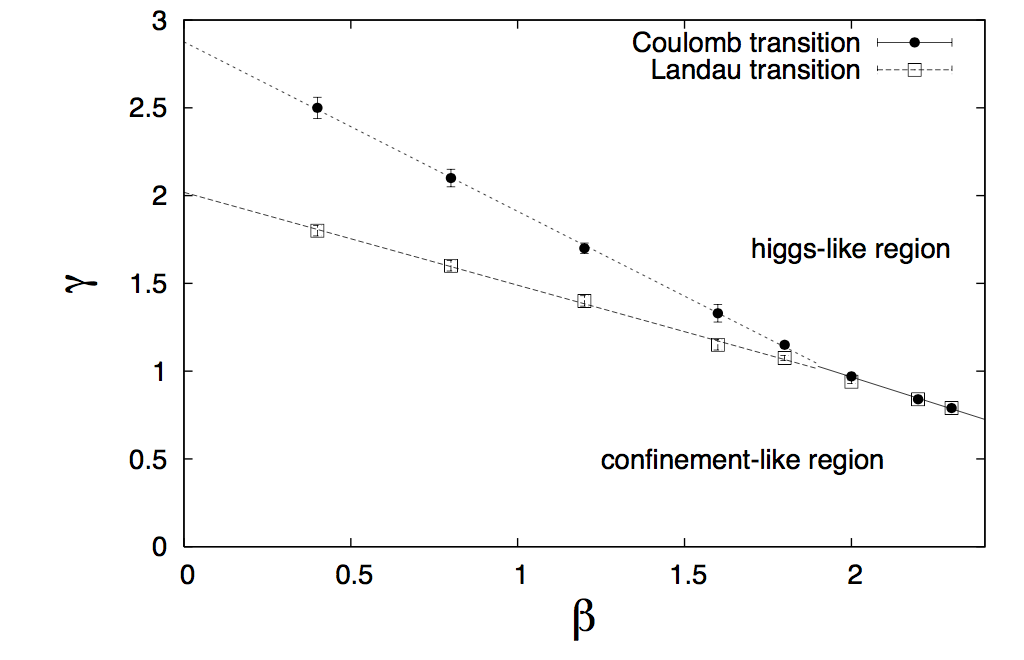
\includegraphics[width=9cm,clip]{pics/SU2H_phase_diagram_GF}
\end{center}
  \caption{Upper panel: sketch of the phase diagram of the SU(2)-Higgs model in the infinite-$\tilde\lambda$ limit. The line of first order phase transitions terminates in the middle of the diagram, indicating that the Higgs and confinement phases are analytically connected.  Both pictures are taken from \cite{Caudy:2007sf}.}
  \label{SU2H_phase_diagram}
\end{figure}




\begin{equation}
\tilde U(t) = \frac{1}{L^3} \sum_{\vec x} U_{0}(\vec x,t)
\end{equation}

\begin{equation}
\mathcal Q_C = \frac{1}{T} \sum_{t=0}^{T-1} \langle \tr [\tilde U(t) \tilde U(t)^{\dagger}] \rangle
\end{equation}

\begin{equation}
\bar S = \frac{1}{TL^3} \sum_{x} S(x)
\end{equation}

\begin{equation}
\mathcal Q_L = \langle \bar S^{\dagger} \bar S \rangle
\end{equation}

\begin{figure}[thb] 
\begin{adjustwidth}{-4em}{-4em}
  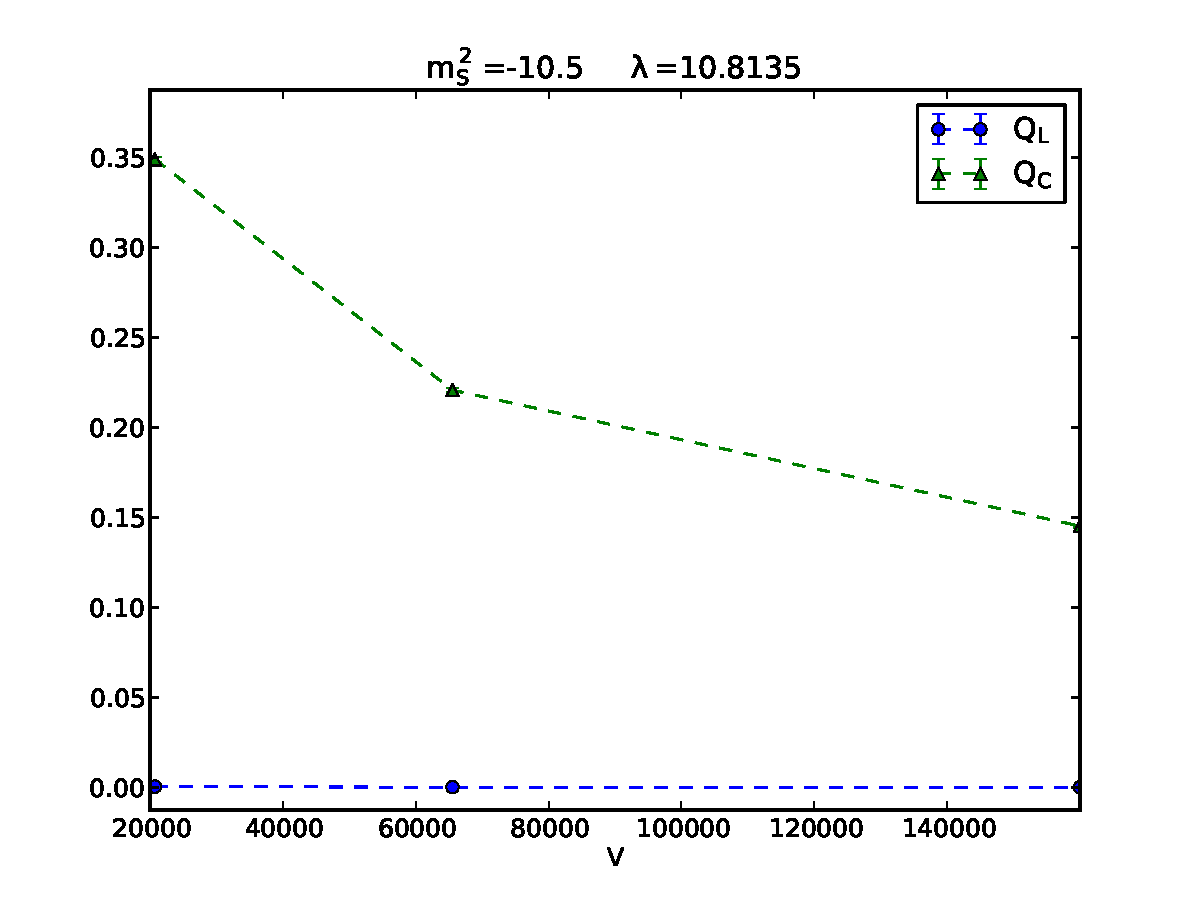
\includegraphics[width=9cm,clip]{pics/SU2H_volume_symm}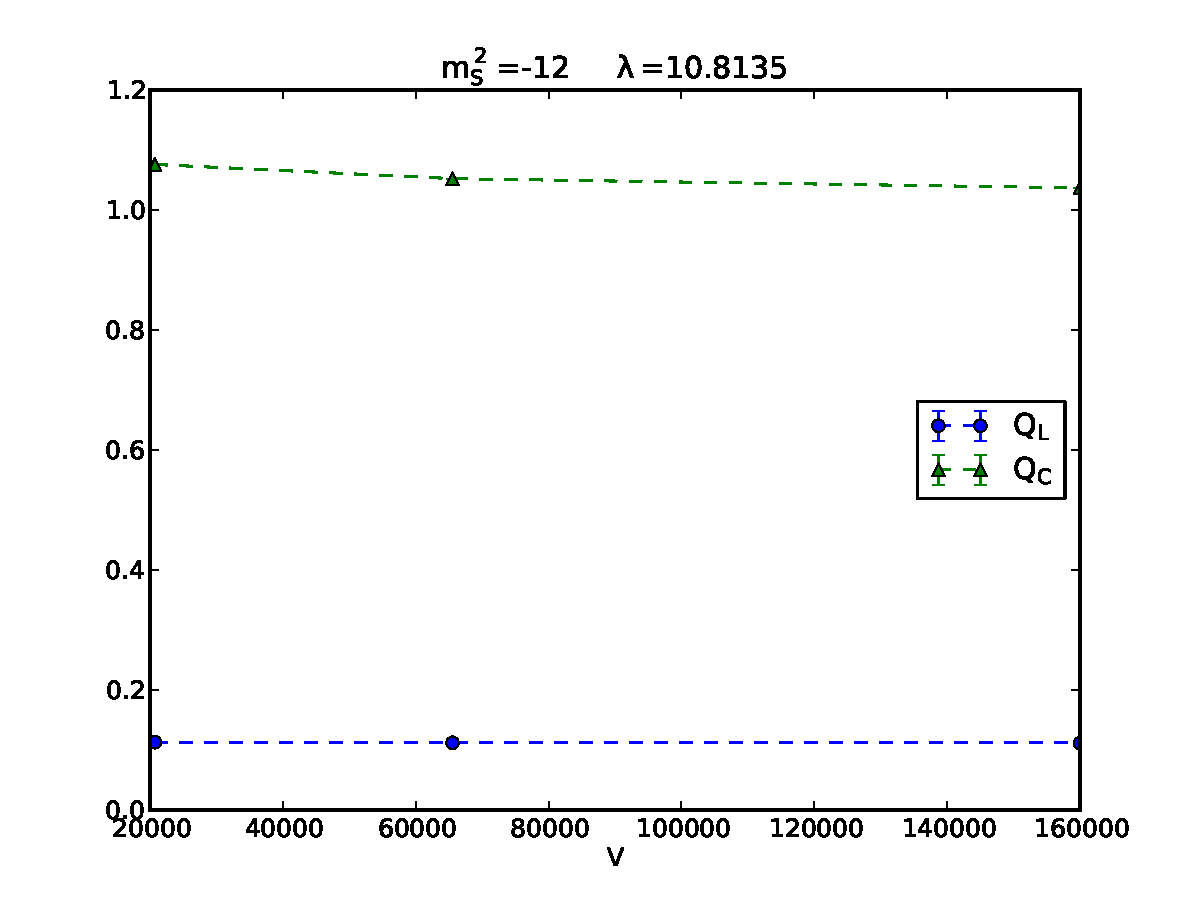
\includegraphics[width=9cm,clip]{pics/SU2H_volume_Higgs}
\end{adjustwidth}
  \caption{.}
  \label{SU2H_volume_scaling}
\end{figure}

We thought it interesting to analyse the behaviour of the gauge-dependent order parameters $\mathcal Q_L$ and $\mathcal Q_C$ in our model with SU(2) gauge symmetry, two fundamental fermions and one fundamental scalar.

\subsection{SU(2)-Higgs model}

As a first step, we considered the SU(2)-Higgs model at $\beta = 2$ and the two different values of $\lambda$ analysed in our study of SU(2) with two fermions and one scalar. We simulated different values of the squared scalar mass $m_S^2$ and measured $\mathcal Q_L$ and $\mathcal Q_C$, plus the scalar condensate $S^{\dagger} S$:

\begin{equation}
S^{\dagger} S = \frac{1}{V} \sum_x S^{\dagger}(x) S(x) \: ,
\end{equation}
%
and the plaquette:

\begin{equation}
U =  \frac{1}{6V} \sum_x \sum_{\mu < \nu} \frac{1}{2} \mathrm{Re} \tr[U_{\mu\nu}(x)] \: .
\end{equation}

We start by reporting the results we obtained at $\lambda = 2$.


\begin{figure}[thb] 
\begin{center}
  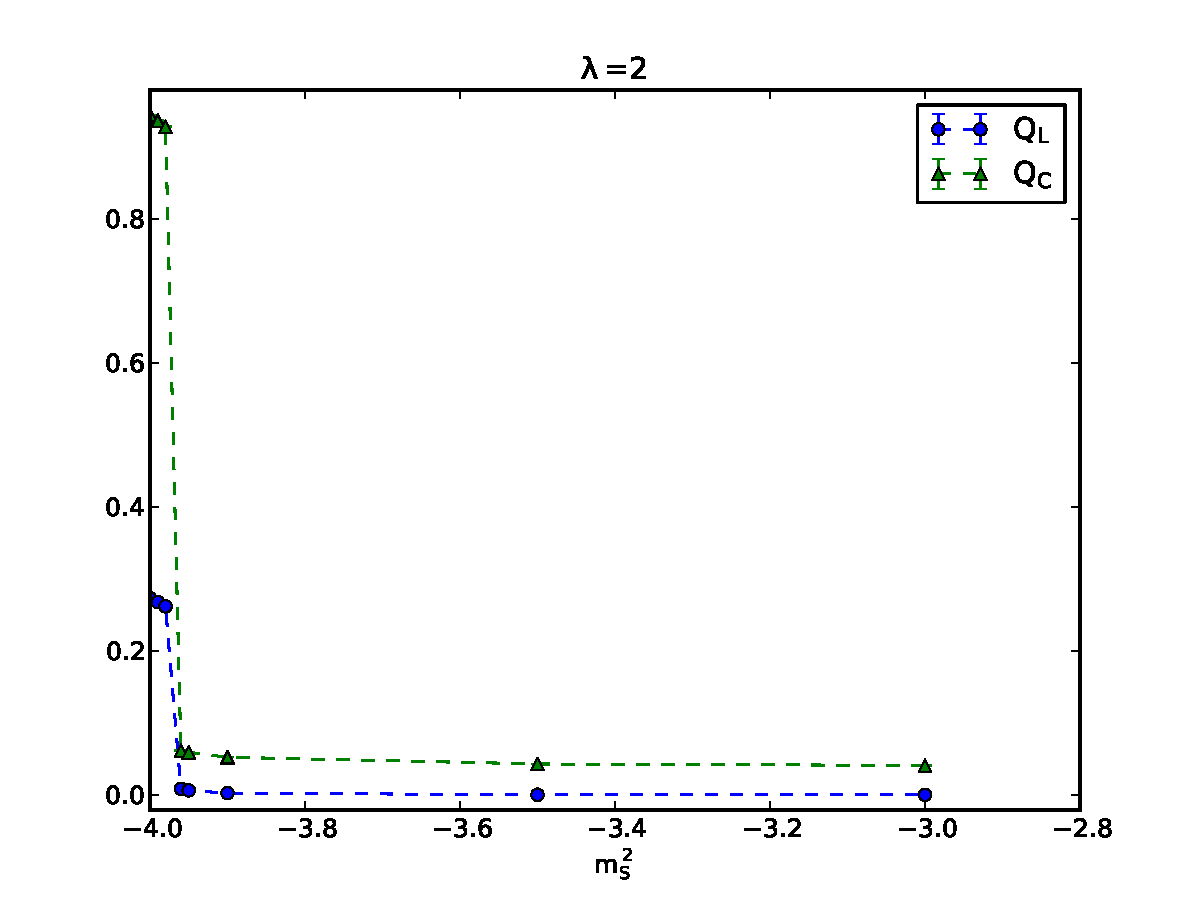
\includegraphics[width=9.5cm,clip]{pics/SU2H_jump_Q}  
  \end{center}
  \caption{.}
  \label{SU2H_jump_Q}
\end{figure}


\begin{figure}[thb] 
\begin{adjustwidth}{-4em}{-4em}
  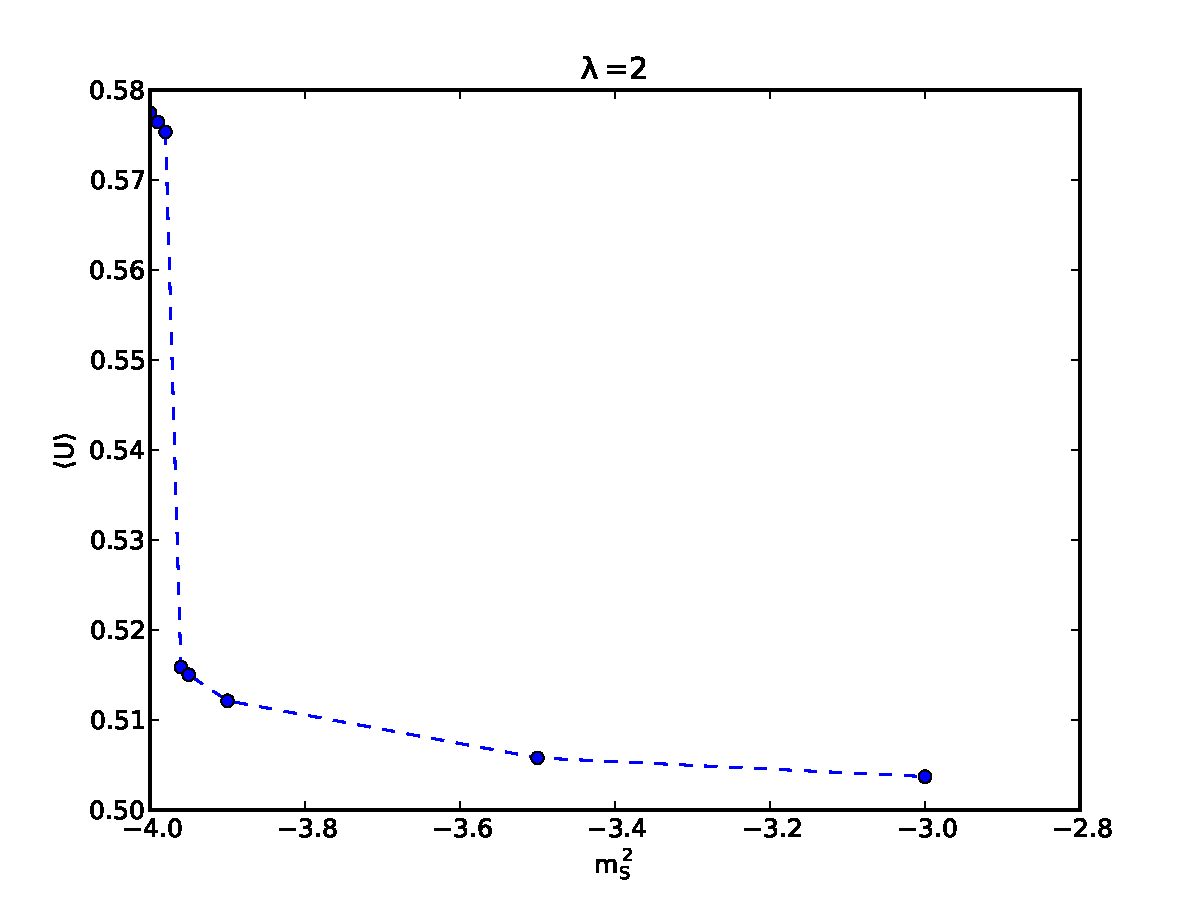
\includegraphics[width=9cm,clip]{pics/SU2H_jump_plaquette}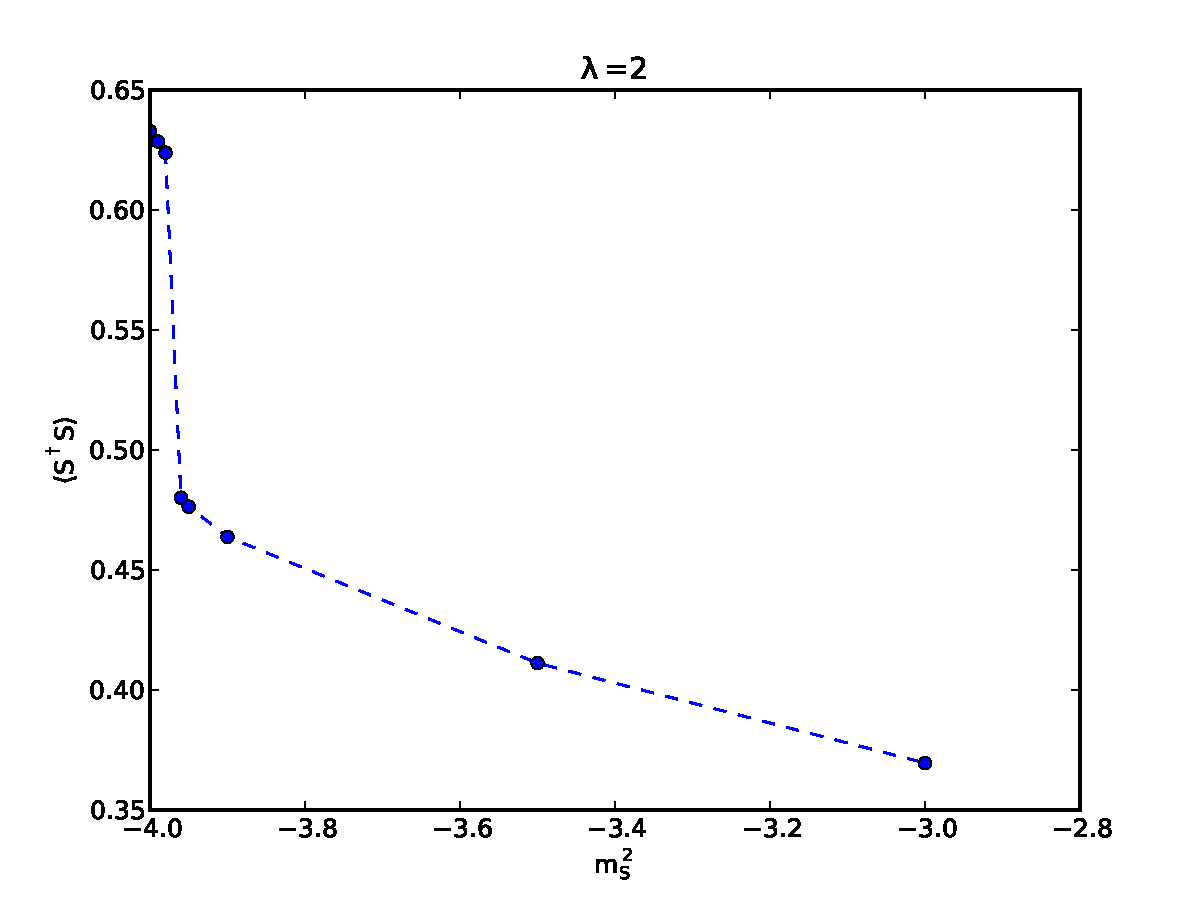
\includegraphics[width=9cm,clip]{pics/SU2H_jump_condensate}
\end{adjustwidth}
  \caption{.}
  \label{SU2H_jump_pl_cond}
\end{figure}



\subsection{SU(2) with fermions and scalars}

\begin{figure}[thb] 
\begin{center}
  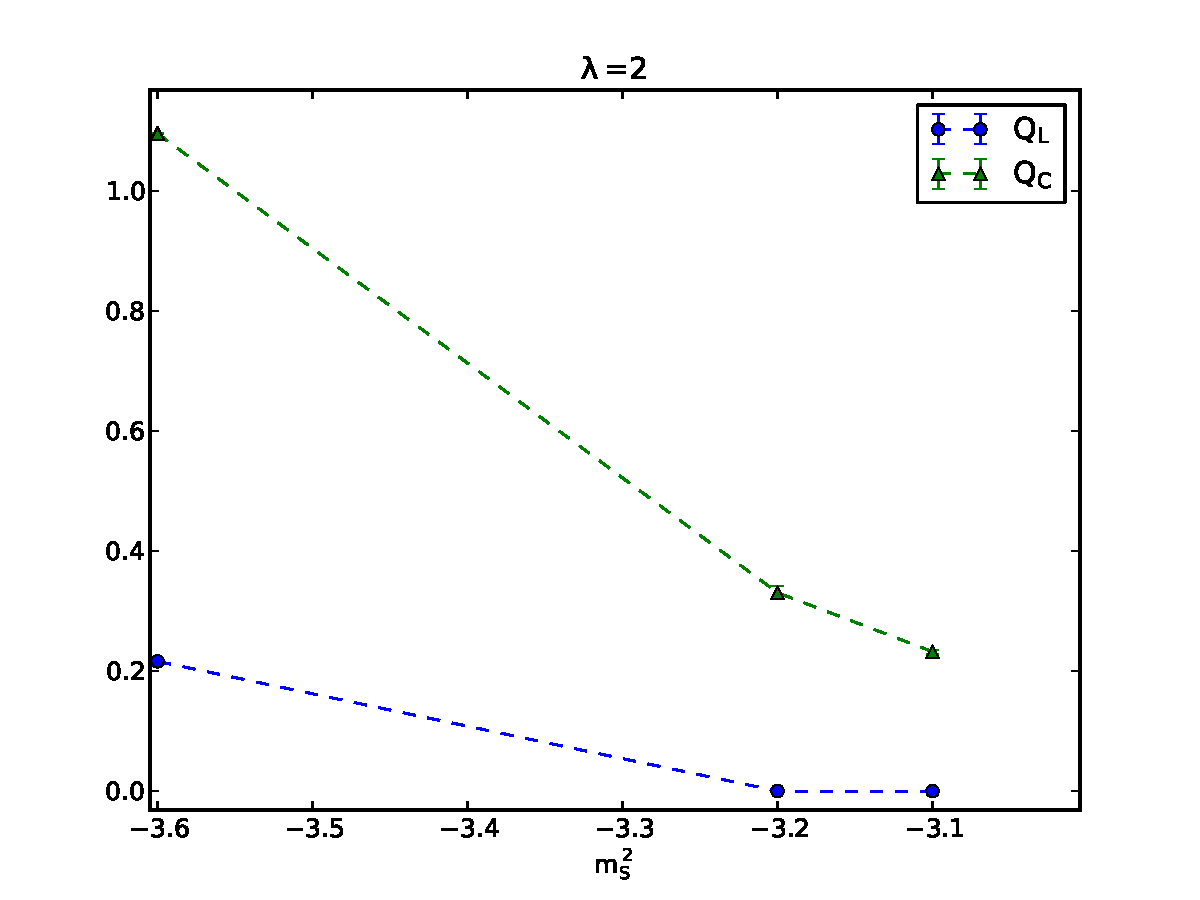
\includegraphics[width=9.5cm,clip]{pics/jump_Q}  
  \end{center}
  \caption{.}
  \label{jump_Q}
\end{figure}

\begin{figure}[thb] 
\begin{adjustwidth}{-4em}{-4em}
  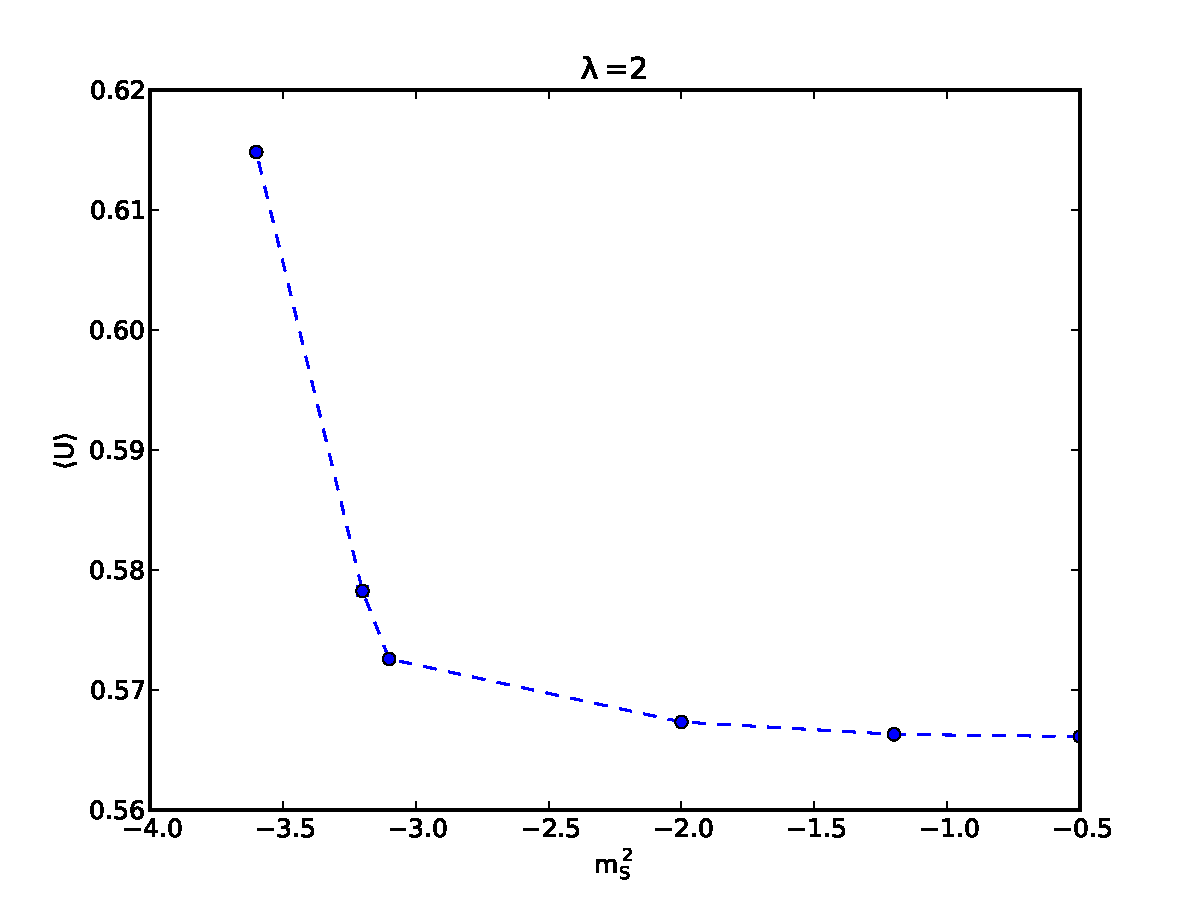
\includegraphics[width=9cm,clip]{pics/jump_plaquette}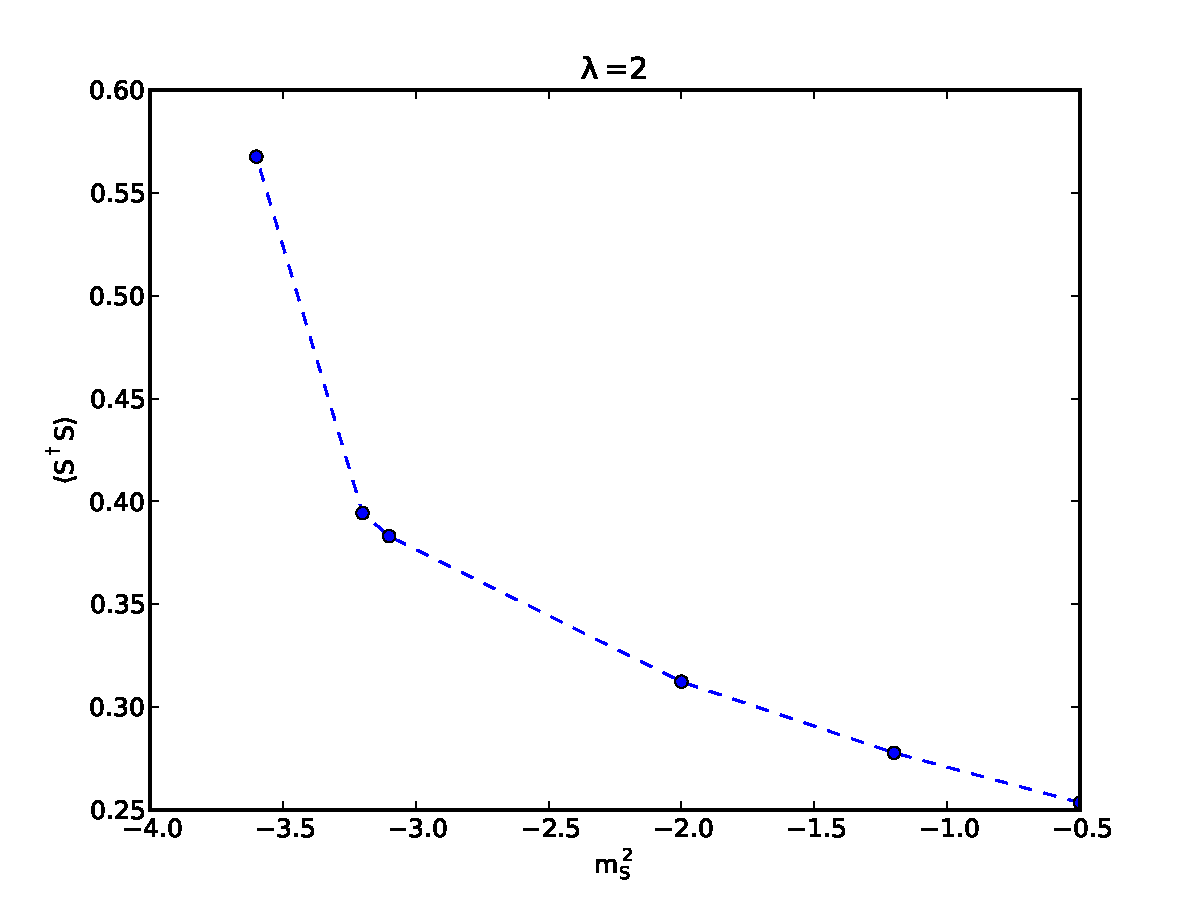
\includegraphics[width=9cm,clip]{pics/jump_condensate}
\end{adjustwidth}
  \caption{.}
  \label{jump_pl_cond}
\end{figure}


%%%%%%%%%%%%%%%%%%%%%%%%%%%%%%%%%%%%%%%%%%%%%%%%%%%%%%

\section{Conclusions and outlook}

%Renormalisation, continuum limit

%%%%%%%%%%%%%%%%%%%%%%%%%%%%%%%%%%%%%%%%%%%%%%%%%%%%%%
